% A LaTeX template for ARTICLE version of the MSc Thesis submissions to 
% Politecnico di Milano (PoliMi) - School of Industrial and Information Engineering
%
% S. Bonetti, A. Gruttadauria, G. Mescolini, A. Zingaro
% e-mail: template-tesi-ingind@polimi.it
%
% Last Revision: October 2021
%
% Copyright 2021 Politecnico di Milano, Italy. Inc. NC-BY

\documentclass[12pt,a4paper]{article} 

%------------------------------------------------------------------------------
%	REQUIRED PACKAGES AND  CONFIGURATIONS
%------------------------------------------------------------------------------
% PACKAGES FOR TITLES
\usepackage{titlesec}
\usepackage{color}

% PACKAGES FOR LANGUAGE AND FONT
\usepackage[utf8]{inputenc}
\usepackage[english]{babel}
\usepackage[T1]{fontenc} % Font encoding

% PACKAGES FOR IMAGES
\usepackage{graphicx}
\graphicspath{{Images/}}
\usepackage{eso-pic} % For the background picture on the title page
\usepackage{subfig} % Numbered and caption subfigures using \subfloat
\usepackage{caption} % Coloured captions
\usepackage{transparent}

% STANDARD MATH PACKAGES
\usepackage{amsmath}
\usepackage{amsthm}
\usepackage{bm}
\usepackage[overload]{empheq}  % For braced-style systems of equations

% PACKAGES FOR TABLES
\usepackage{tabularx}
\usepackage{longtable} % tables that can span several pages
\usepackage{colortbl}

% PACKAGES FOR ALGORITHMS (PSEUDO-CODE)
\usepackage{algorithm}
\usepackage{algorithmic}

% PACKAGES FOR REFERENCES & BIBLIOGRAPHY
\usepackage[colorlinks=true,linkcolor=black,anchorcolor=black,citecolor=black,filecolor=black,menucolor=black,runcolor=black,urlcolor=black]{hyperref} % Adds clickable links at references
\usepackage{cleveref}
\usepackage[square, numbers, sort&compress]{natbib} % Square brackets, citing references with numbers, citations sorted by appearance in the text and compressed
\bibliographystyle{plain} % You may use a different style adapted to your field

% PACKAGES FOR THE APPENDIX
\usepackage{appendix}

% PACKAGES FOR ITEMIZE & ENUMERATES 
\usepackage{enumitem}

% OTHER PACKAGES
\usepackage{amsthm,thmtools,xcolor} % Coloured "Theorem"
\usepackage{comment} % Comment part of code
\usepackage{fancyhdr} % Fancy headers and footers
\usepackage{lipsum} % Insert dummy text
\usepackage{tcolorbox} % Create coloured boxes (e.g. the one for the key-words)

\usepackage{amsmath}
\usepackage{amsthm}
\usepackage{amssymb}
\usepackage{amsfonts}
\usepackage{bm}
\usepackage[overload]{empheq} % For braced-style systems of equations.
\usepackage{fix-cm} % To override original LaTeX restrictions on sizes
\usepackage{siunitx}

\usepackage{minted}
\usepackage{cprotect}

%-------------------------------------------------------------------------
%	NEW COMMANDS DEFINED
%-------------------------------------------------------------------------
% EXAMPLES OF NEW COMMANDS -> here you see how to define new commands
\newcommand{\bea}{\begin{eqnarray}} % Shortcut for equation arrays
\newcommand{\eea}{\end{eqnarray}}
\newcommand{\e}[1]{\times 10^{#1}}  % Powers of 10 notation
\newcommand{\mathbbm}[1]{\text{\usefont{U}{bbm}{m}{n}#1}} % From mathbbm.sty
\newcommand{\pdev}[2]{\frac{\partial#1}{\partial#2}}
% NB: you can also override some existing commands with the keyword \renewcommand

%----------------------------------------------------------------------------
%	ADD YOUR PACKAGES (be careful of package interaction)
%----------------------------------------------------------------------------


%----------------------------------------------------------------------------
%	ADD YOUR DEFINITIONS AND COMMANDS (be careful of existing commands)
%----------------------------------------------------------------------------


% Do not change Configuration_files/config.tex file unless you really know what you are doing. 
% This file ends the configuration procedures (e.g. customizing commands, definition of new commands)
% Configuration package
\usepackage[bottom=2.0cm,top=2.0cm,left=2.0cm,right=2.0cm]{geometry}
\raggedbottom 

% Create color bluePoli (-> manuale grafica coordinata:  https://www.polimi.it/fileadmin/user_upload/il_Politecnico/grafica-coordinata/2015_05_11_46xy_manuale_grafica_coordinata.pdf)
\definecolor{bluePoli}{cmyk}{0.4,0.1,0,0.4}

% Custom theorem environments
\declaretheoremstyle[
  headfont=\color{bluePoli}\normalfont\bfseries,
  bodyfont=\color{black}\normalfont\itshape,
]{colored}

\captionsetup[figure]{labelfont={color=bluePoli}} % Set colour of the captions
\captionsetup[table]{labelfont={color=bluePoli}} % Set colour of the captions
\captionsetup[algorithm]{labelfont={color=bluePoli}} % Set colour of the captions

\theoremstyle{colored}
\newtheorem{theorem}{Theorem}[section]
\newtheorem{proposition}{Proposition}[section]

% Enhances the features of the standard "table" and "tabular" environments.
\newcommand\T{\rule{0pt}{2.6ex}}
\newcommand\B{\rule[-1.2ex]{0pt}{0pt}}

% Algorithm description
\newcounter{algsubstate}
\renewcommand{\thealgsubstate}{\alph{algsubstate}}
\newenvironment{algsubstates}{
    \setcounter{algsubstate}{0}%
    \renewcommand{\STATE}{%
    \stepcounter{algsubstate}%
    \Statex {\small\thealgsubstate:}\space}
    }{}
    
% Custom theorem environment
\newcolumntype{L}[1]{>{\raggedright\let\newline\\\arraybackslash\hspace{0pt}}m{#1}}
\newcolumntype{C}[1]{>{\centering\let\newline\\\arraybackslash\hspace{0pt}}m{#1}}
\newcolumntype{R}[1]{>{\raggedleft\let\newline\\\arraybackslash\hspace{0pt}}m{#1}}

% Custom itemize environment
\setlist[itemize,1]{label=$\bullet$}
\setlist[itemize,2]{label=$\circ$}
\setlist[itemize,3]{label=$-$}
\setlist{nosep}

% Create command for background pic
\newcommand\BackgroundPic{% Adding background picture
	\put(237,365){
	    \parbox[b][\paperheight]{\paperwidth}{%
	    \vfill
		\centering
		\transparent{0.4}
		
\includegraphics[width=0.44\paperwidth]{raggiera_polimi.eps}%
		\vfill}
		}
}

% Set indentation
\setlength\parindent{0pt}

% Custom title commands
\titleformat{\section}
{\color{bluePoli}\normalfont\Large\bfseries}
{\color{bluePoli}\thesection.}{1em}{}
\titlespacing*{\section}
{0pt}{3.3ex}{3.3ex}

\titleformat{\subsection}
{\color{bluePoli}\normalfont\large\bfseries}
{\color{bluePoli}\thesubsection.}{1em}{}
\titlespacing*{\subsection}
{0pt}{3.3ex}{3.3ex}

% Custom headers and footers
\pagestyle{fancy}
\fancyhf{}
      
\fancyfoot{}
\fancyfoot[C]{\thepage} % page
\renewcommand{\headrulewidth}{0mm} % headrule width
\renewcommand{\footrulewidth}{0mm} % footrule width

\makeatletter
\patchcmd{\headrule}{\hrule}{\color{black}\hrule}{}{} % headrule
\patchcmd{\footrule}{\hrule}{\color{black}\hrule}{}{} % footrule
\makeatother

% Insert here the info that will be displayed into your Title page 
% -> title of your work
\renewcommand{\title}{Homework Report}
% -> author name and surname
\renewcommand{\author}{Giovanni Versiglioni}
% -> MSc course
\newcommand{\course}{Computer Science and Engineering}
% -> advisor name and surname
%\newcommand{\advisor}{Prof. Name Surname}
% IF AND ONLY IF you need to modify the co-supervisors you also have to modify the file Configuration_files/title_page.tex (ONLY where it is marked)
%\newcommand{\firstcoadvisor}{Name Surname} % insert if any otherwise comment
%\newcommand{\secondcoadvisor}{Name Surname} % insert if any otherwise comment
% -> author ID
\newcommand{\ID}{11015537}
% -> academic year
\newcommand{\YEAR}{2023-2024}
% -> abstract (only in English)
\renewcommand{\abstract}{}

% -> key-words (only in English)
\newcommand{\keywords}{here, the keywords, of your thesis}

\counterwithin{figure}{section}

\usepackage{forest}

\definecolor{folderbg}{RGB}{124,166,198}
\definecolor{folderborder}{RGB}{110,144,169}

\def\Size{4pt}
\tikzset{
      folder/.pic={
        \filldraw[draw=folderborder,top color=folderbg!50,bottom color=folderbg]
          (-1.05*\Size,0.2\Size+5pt) rectangle ++(.75*\Size,-0.2\Size-5pt);  
        \filldraw[draw=folderborder,top color=folderbg!50,bottom color=folderbg]
          (-1.15*\Size,-\Size) rectangle (1.15*\Size,\Size);
      }
    }

% DOCUMENT START
\begin{document}

\nocite{bookCV}

% DO NOT REMOVE SPACES BETWEEN LINES!

\AddToShipoutPicture*{\BackgroundPic}

\hspace{-0.6cm}
\includegraphics[width=0.6\textwidth]{logo_polimi_ing_indinf.eps}

\vspace{-1mm}
\Large{\textbf{\color{bluePoli}{\title}}}\\

\vspace{-0.2cm}
\fontsize{0.3cm}{0.5cm}\selectfont \bfseries \textsc{\color{bluePoli} Image Analysis and Computer Vision, 2023-2024 \\ \course}\\

\vspace{-0.2cm}
\large{\textbf{\author, \ID}}

\small \normalfont

\vspace{11pt}

\centerline{\rule{1.0\textwidth}{0.4pt}}

%\begin{center}
%\begin{minipage}[t]{.24\textwidth}
%\begin{minipage}{.90\textwidth}
%\noindent
%\scriptsize{\textbf{Advisor:}} \\
%\advisor \\
%\\
%\textbf{Co-advisors:} \\ % leave it if any co-advisor otherwise comment
%\firstcoadvisor \\ % leave it if any co-advisor otherwise comment
%\secondcoadvisor \\ % leave it if you have more that one co-advisor otherwise comment (if you have more than two co-advisors just copy&paste this line writing \thirdcoadvisor, \fourthcoadvisor, ecc. (REMEMBER to modify also the main.txt)
%\\ % leave it if any co-advisor otherwise comment
%\textbf{Academic year:} \\
%\YEAR \\
%\\
%\end{minipage}
%\end{minipage}% This must go next to `\end{minipage}`
%\begin{minipage}{.74\textwidth}
%\noindent \textbf{\color{bluePoli} Abstract:} {\abstract}
%\end{minipage}
%\end{center}

%\vspace{15pt}

%\begin{tcolorbox}[arc=0pt, boxrule=0pt, colback=bluePoli!60, width=\textwidth, colupper=white]
    %\textbf{Key-words:} \keywords
%\end{tcolorbox}

\vspace{12pt}

\setcounter{section}{-1}

\tableofcontents
\listoffigures

\section{Introduction}
\label{sec:introduction}
This is the report for the Image Analysis and Computer Vision Homework, A.Y. 2023-2024.\\

\textbf{Scene (Figure \ref{fig:cylinder}).} A right circular cylinder together with two circular cross sections and two generatrix lines. A right circular cylinder is a surface, made of parallel lines, which is
symmetric about a symmetry axis. A circular cross section of a right cylinder is a circumference
centered on the symmetry axis and perpendicular to the symmetry axis. A generatrix line is a
straight line, on the cylinder surface, which is parallel to its axis.\\

\textbf{Image (Figure \ref{fig:palazzoTe}).} A single image is taken of the described cylinder by an uncalibrated, zero-skew camera. Two circular cross sections are visible, and their images $C_1,C_2$ are extracted. Two (parallel) generatrix lines of the cylinder are also visible, and their images $l_1,l_2$ are extracted.

\begin{figure}[H]
    \centering
    \subfloat[Scene -- Right circular cylinder with two cross sections and two generatrix lines.\label{fig:cylinder}]{
        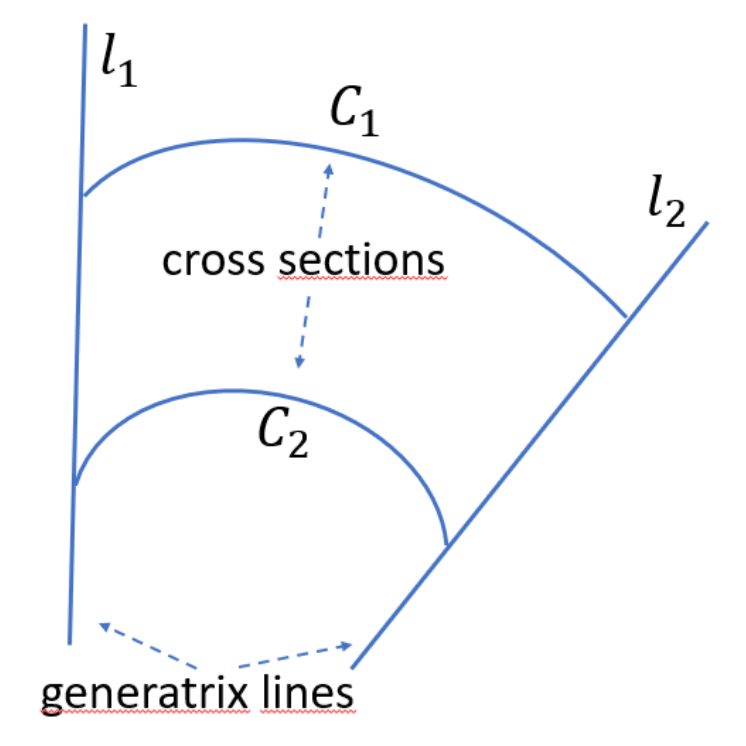
\includegraphics[width=0.47\textwidth]{Images/Cylinder.png}
    }
    \quad
    \subfloat[Image -- Cylindrical voult in Palazzo Te, Mantova, Italy.\label{fig:palazzoTe}]{
        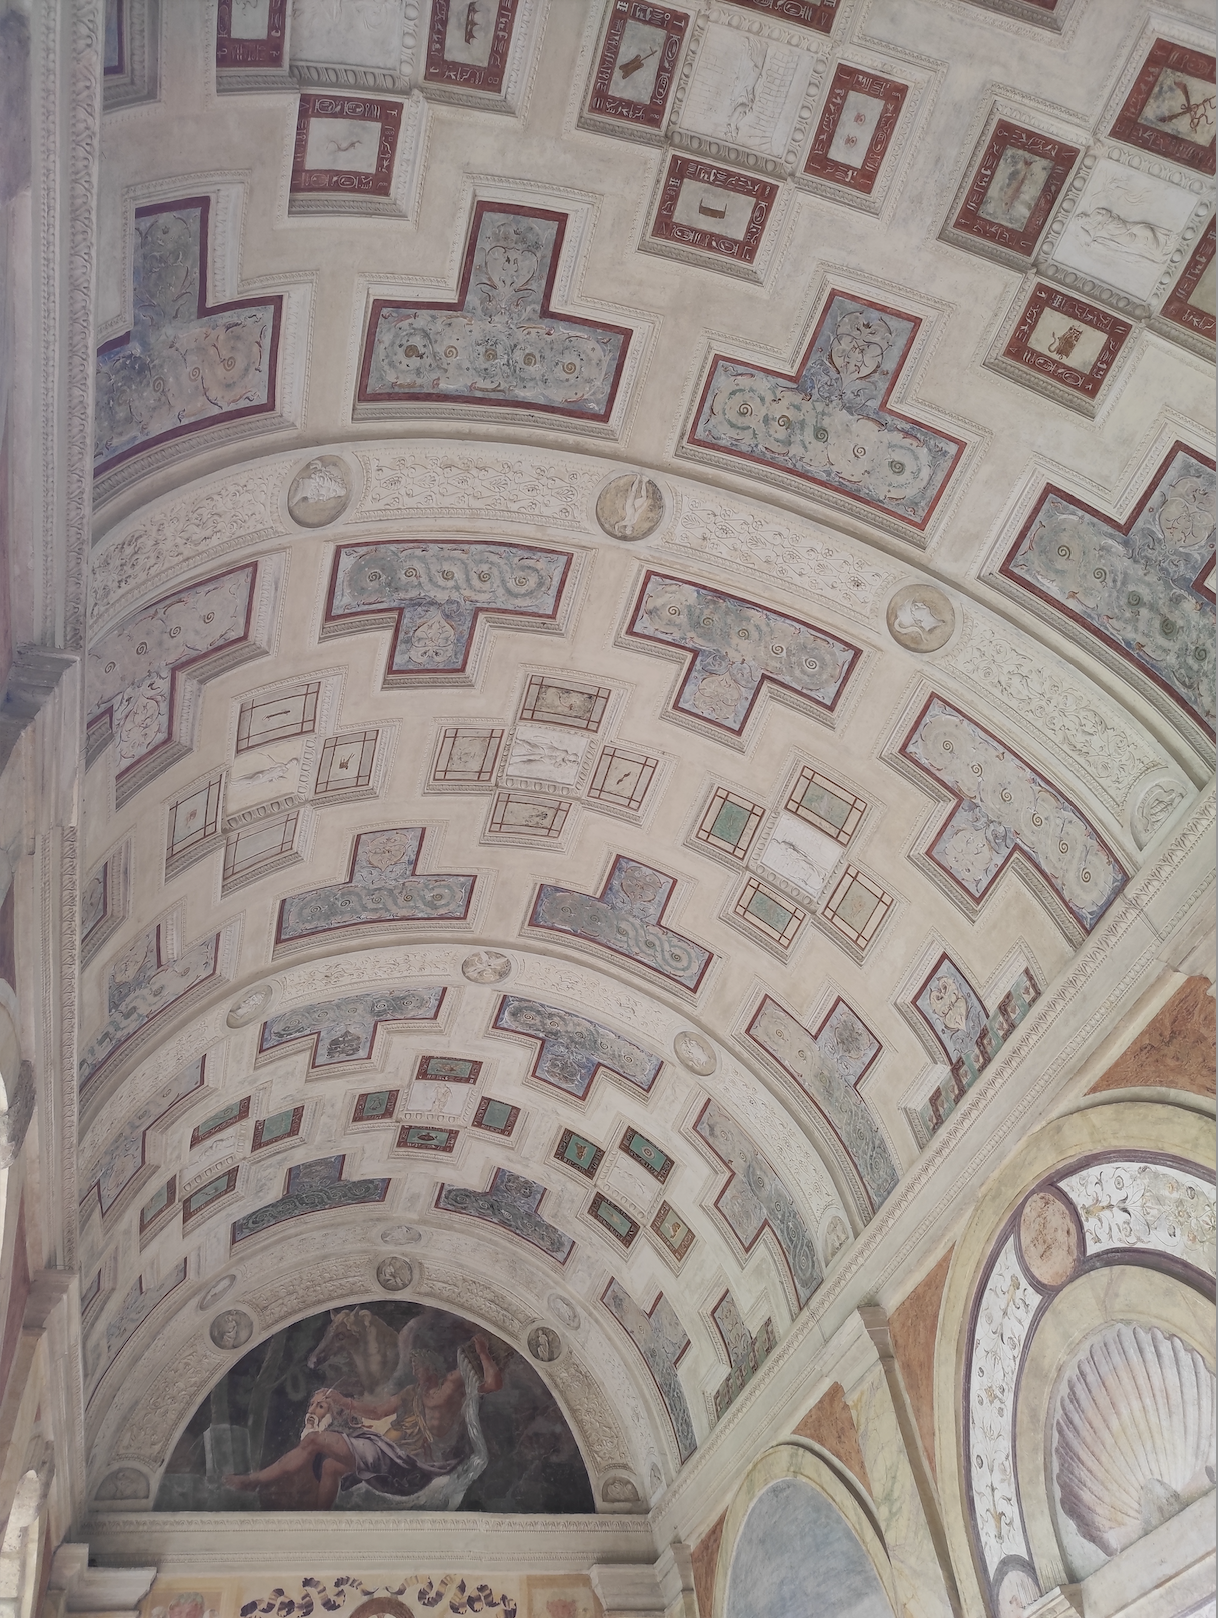
\includegraphics[width=0.47\textwidth]{Images/PalazzoTe.png}
    }
    \caption[Homework problem formulation and image data.]{Homework problem formulation and image data.}
    \label{fig:problem}
\end{figure}

\section{Feature Extraction}
\label{sec:featureExtraction}
The goal is to retrieve geometrical data -- such as edges, corners, and lines -- from the given image.

\subsection{Edge Detection}
\label{sec:edgeDetection}
The \textbf{Canny} method can be used to detect edges in the image.\\

The algorithm comprises the following sequential steps:
\begin{itemize}
    \item[(i)] Apply Gaussian filter to smooth the image in order to remove noise;
    \item[(ii)] Find the intensity gradients of the image;
    \item[(iii)] Apply gradient magnitude thresholding or lower bound cut-off suppression to get rid of spurious response to edge detection;
    \item[(iv)] Apply double threshold to determine potential edges;
    \item[(v)] Track edges by hysteresis (i.e. finalize the detection of edges by suppressing all the other edges that are weak and not connected to strong edges).
\end{itemize}
\bigskip
MATLAB already includes -- in the Image Processing Toolbox -- an implementation of this method in the \verb|edge| function, which has been used in the \verb|detectEdges.m| script. \textbf{Figure \ref{fig:edges}} shows the resulting image.

\begin{figure}[H]
    \centering
    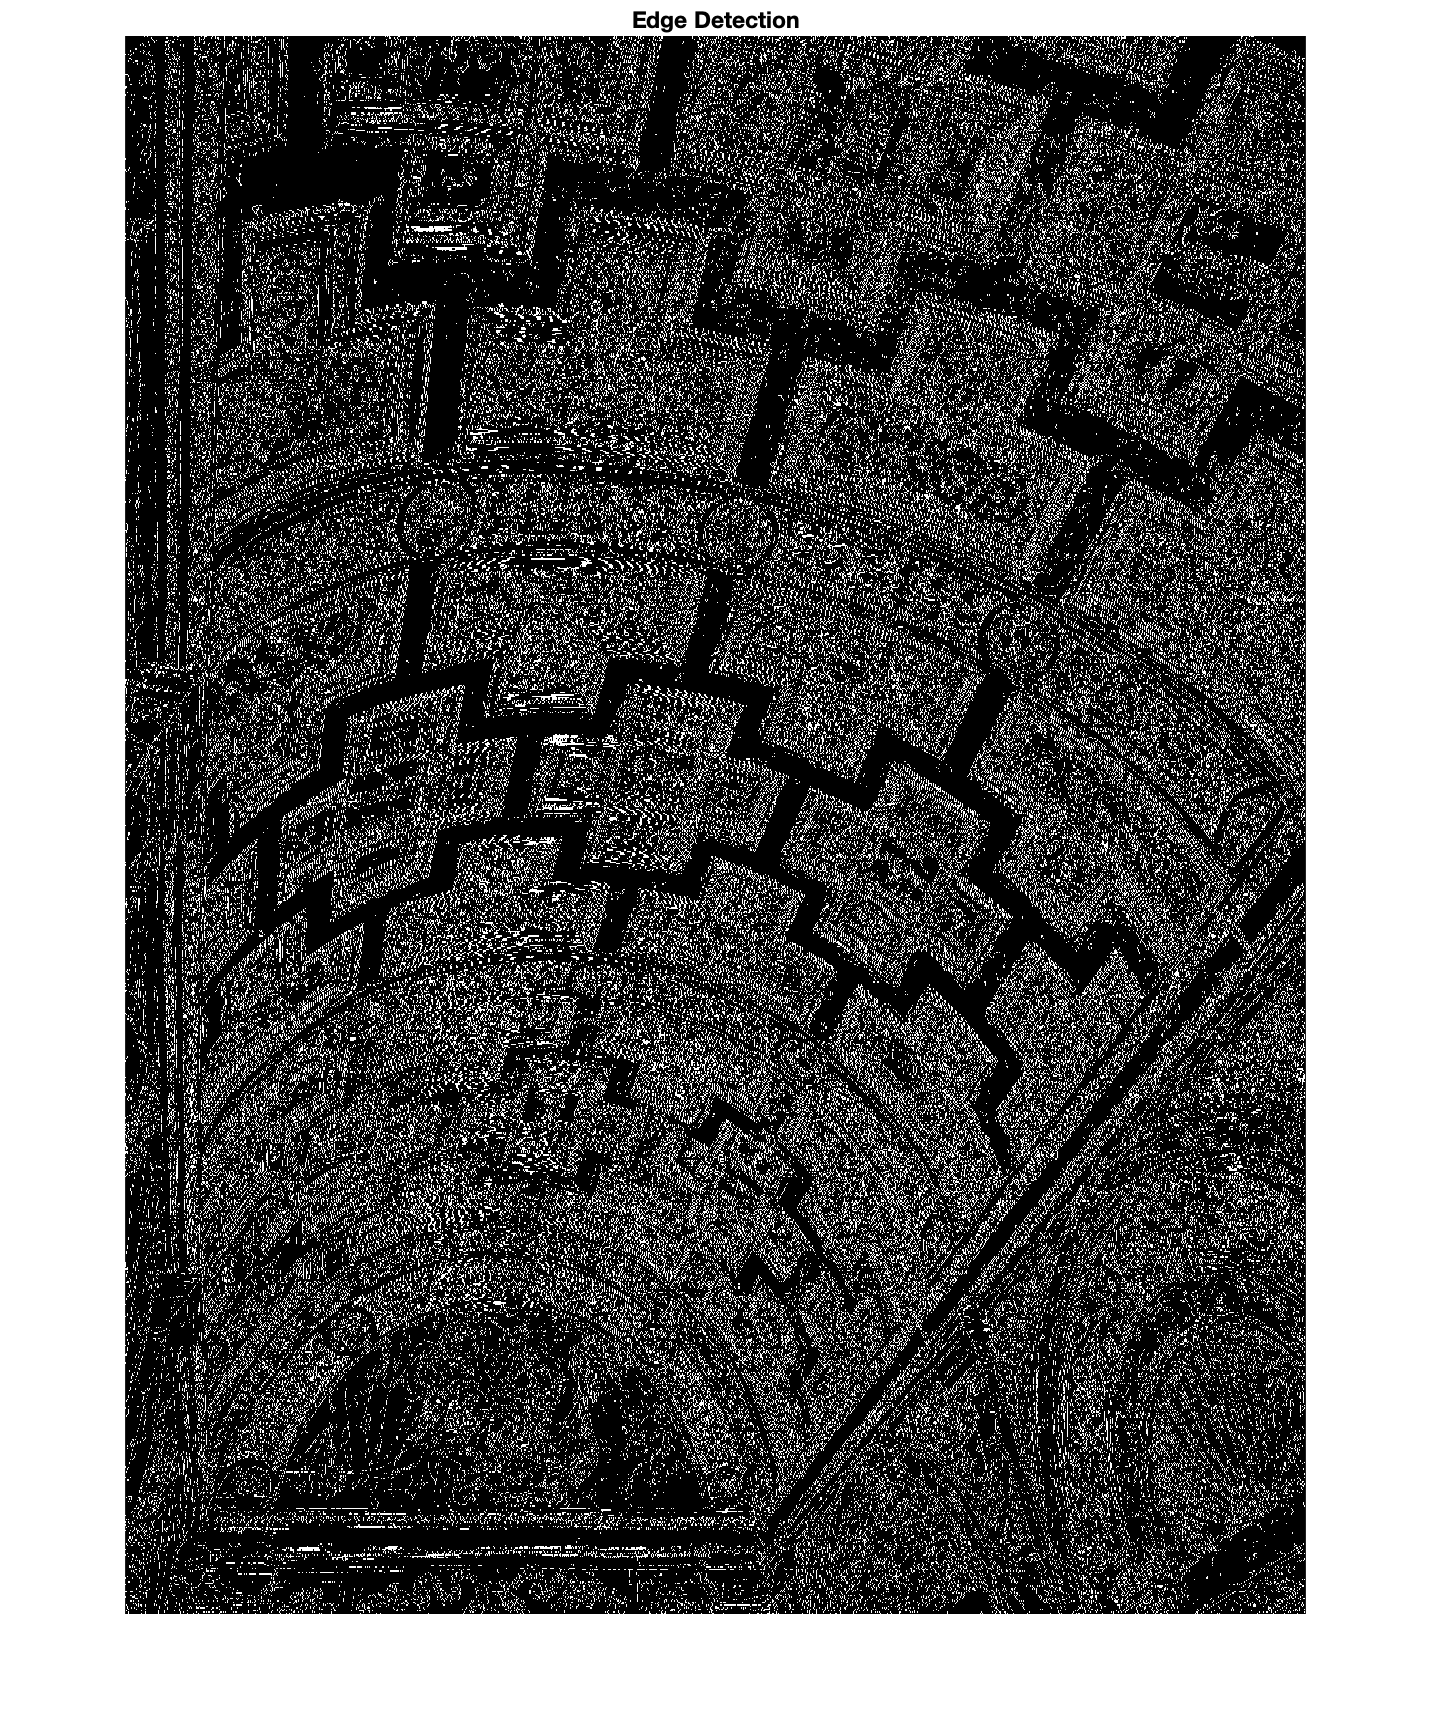
\includegraphics[width=0.9\textwidth]{Images/PalazzoTe_edges.png}
    \caption[Edge Detection -- Canny Method.]{Edge Detection -- Canny Method.}
    \label{fig:edges}
\end{figure}

\subsection{Corner Detection}
\label{sec:cornerDetection}
The \textbf{Harris} method can be used to detect corners in the image.\\

The algorithm comprises the following sequential steps:
\begin{itemize}
    \item[(i)] Color to gray-scale in order to work on a single channel and enhancing speed processing;
    \item[(ii)] Spatial derivative calculation to highlight pattern changes around each pixel region analyzed and then setting up the tensor structure;
    \item[(iii)] Harris response calculation by computing the smallest approximated eigenvalue of the structure tensor;
    \item[(iv)] Non-maximum suppression in order to pick up the optimal values to indicate corners -- find the local maxima as corners within the window which is a 3 by 3 filter.
\end{itemize}
\bigskip
The function \verb|findCorners.m| implements this method and is used in the \verb|detectCorners.m| script to compute corners in the image. \textbf{Figure \ref{fig:corners}} shows the resulting image.

\begin{figure}[H]
    \centering
    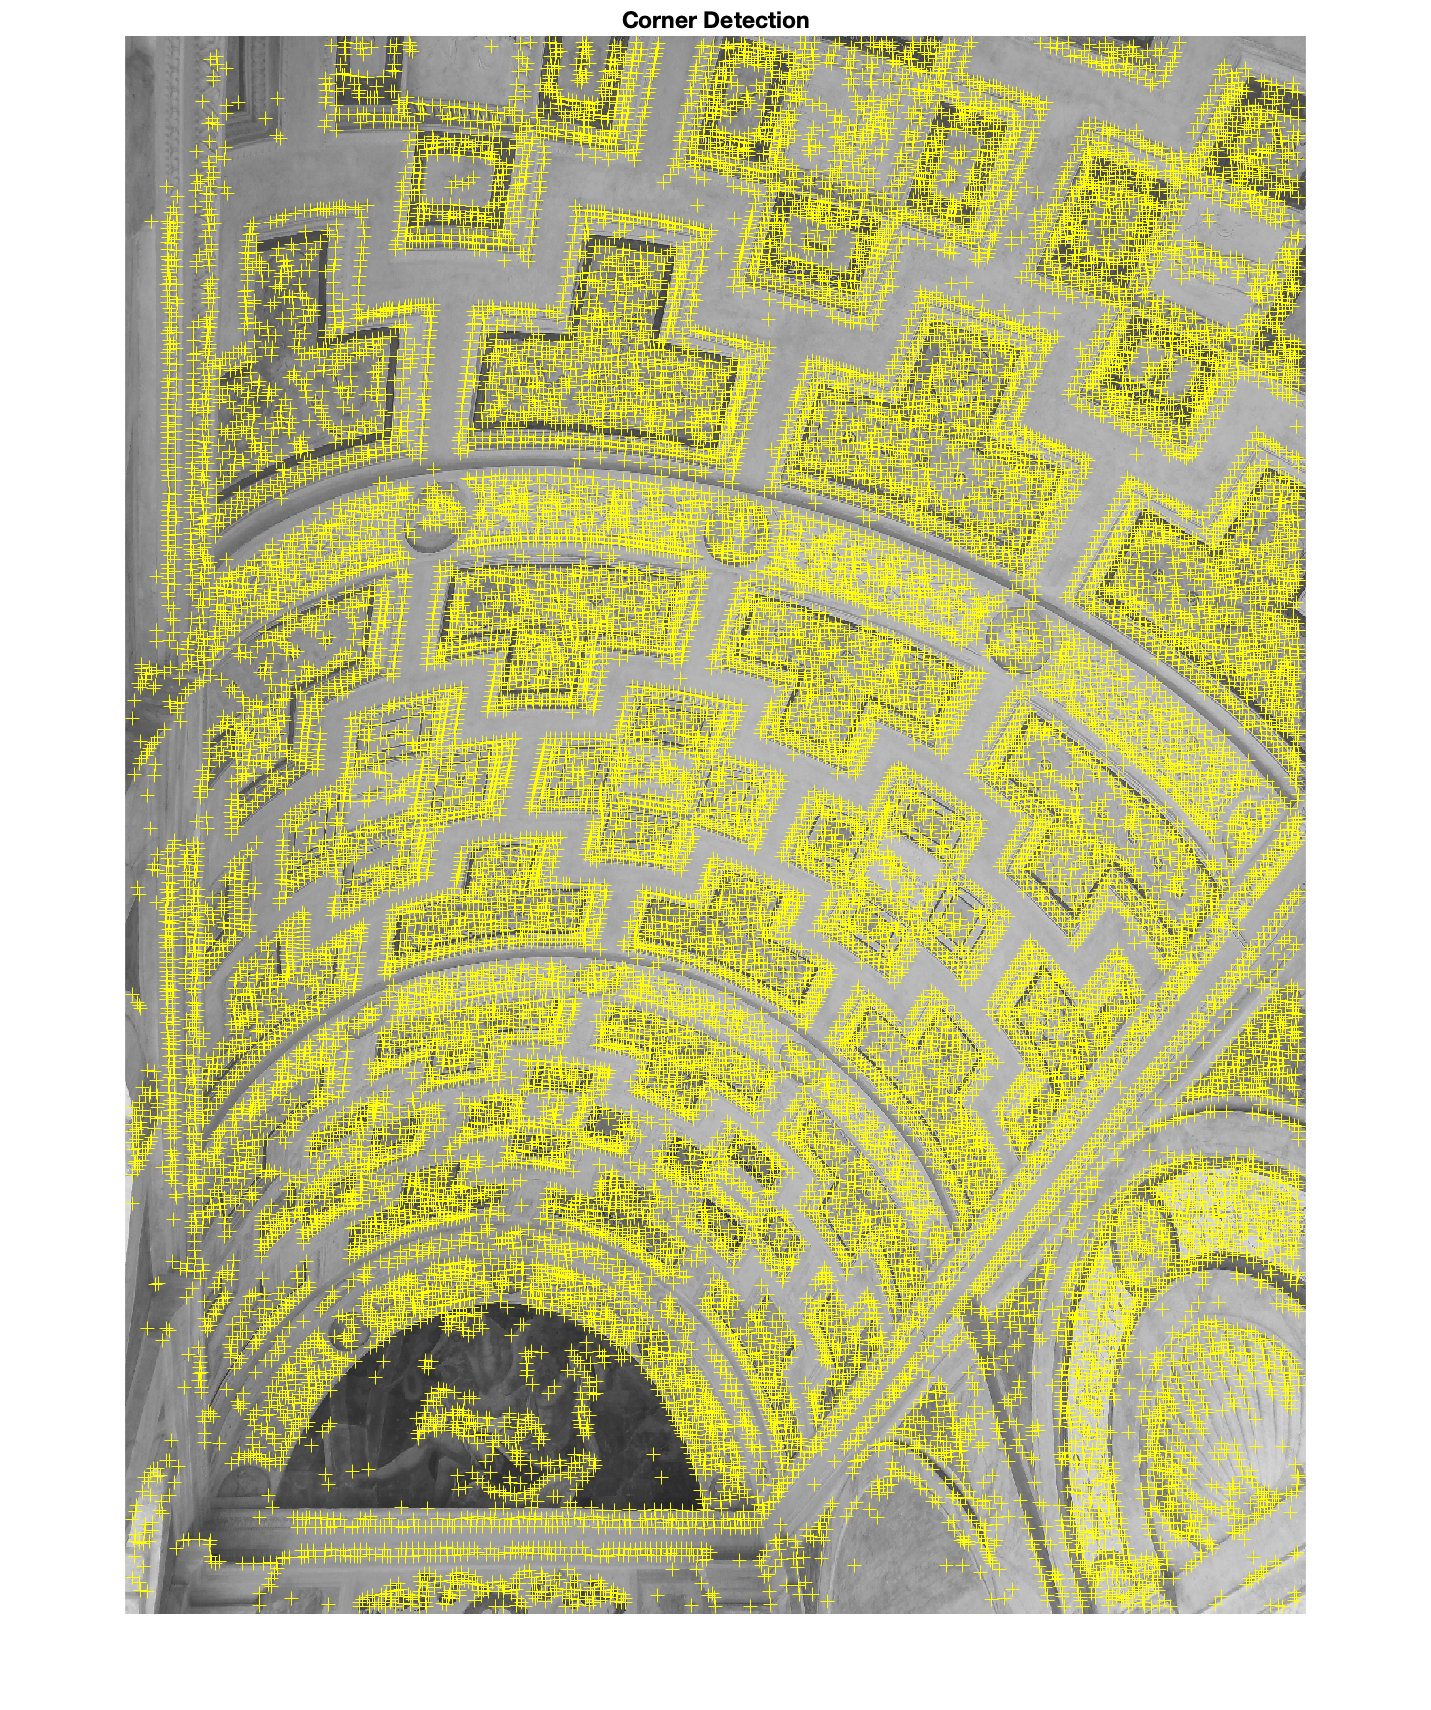
\includegraphics[width=0.83\textwidth]{Images/PalazzoTe_corners.png}
    \caption[Corner Detection -- Harris Method.]{Corner Detection -- Harris Method.}
    \label{fig:corners}
\end{figure}

\subsection{Line Detection}
\label{sec:lineDetection}
The \textbf{Hough Transform} method can be used to detect lines in the image.\\

The algorithm comprises the following steps:
\begin{itemize}
    \item[(i)] Edge detection: using the Canny edge detector;
    \item[(ii)] Mapping of edge points to the Hough space and storage in an accumulator;
    \item[(iii)] Interpretation of the accumulator to yield lines of infinite length (interpretation is done by thresholding and possibly other constraints);
    \item[(iv)] Conversion of infinite lines to finite lines based on the hyper-parameters setting.
\end{itemize}
\bigskip
The function \verb|findLines.m| implements this method and is used in the \verb|detectLines.m| script to compute lines in the image. \textbf{Figure \ref{fig:lines}} shows the resulting image.

\begin{figure}[H]
    \centering
    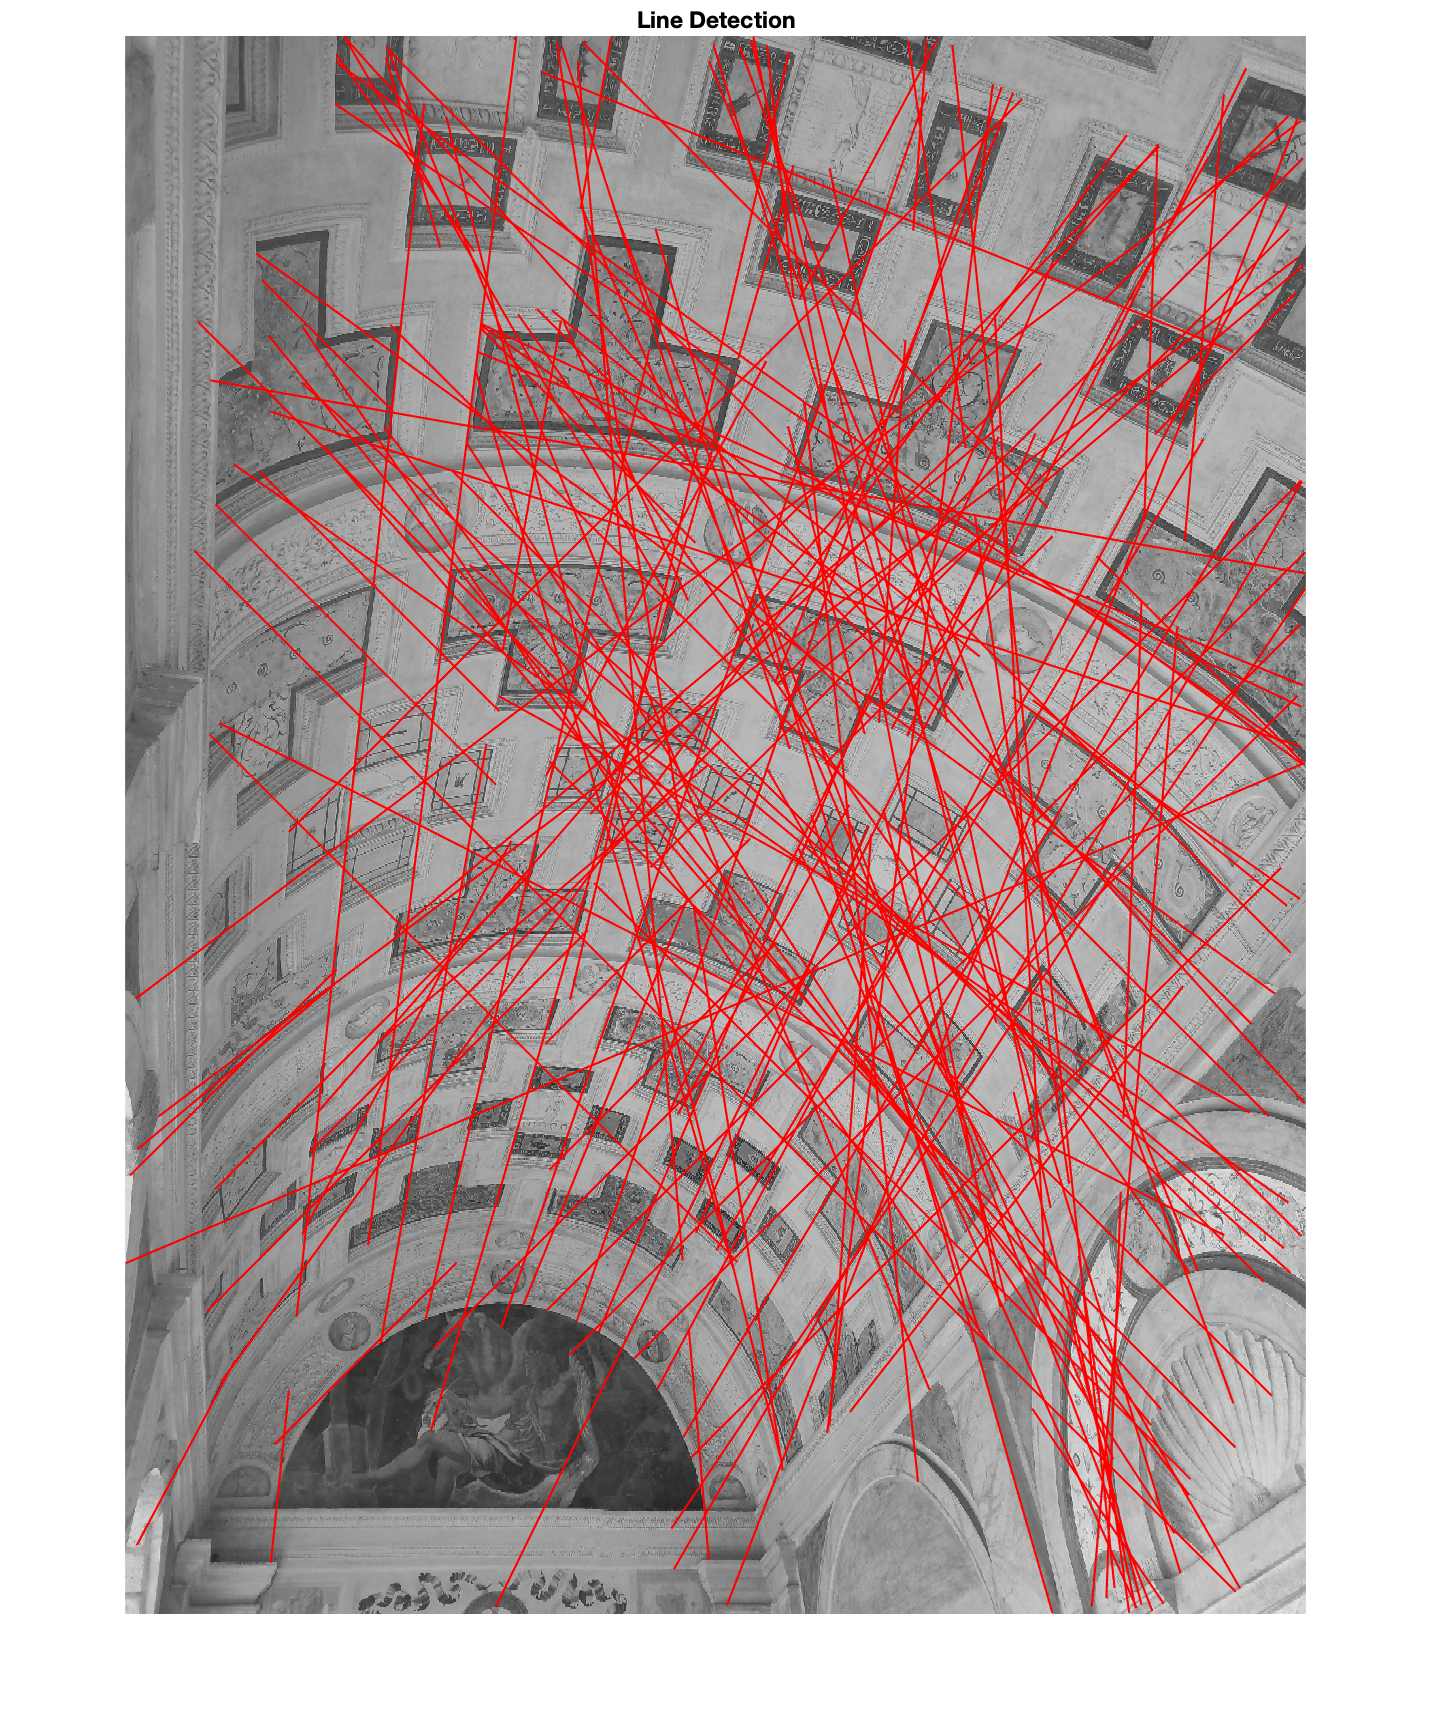
\includegraphics[width=0.83\textwidth]{Images/PalazzoTe_lines.png}
    \caption[Line Detection -- Hough Transform.]{Line Detection -- Hough Transform.}
    \label{fig:lines}
\end{figure}

\section{Rectification}
\label{sec:reconstruction}
This section comprises two main parts. The first part presents theoretical results to Problems 1-5 computed in MATLAB. In the second part will be carried out the metric rectification of a cylindrical surface. Specifically, the unfolding of the part of the surface included between two cross section will be reconstructed onto a plane.

\subsection{Problems}
\label{sec:problems}
The script \verb|Problems.m| contains all the proceedings and results of the following theoretical problems:
\begin{enumerate}
    \item From $C_1,C_2$ find the horizon (vanishing) line $h$ of the plane orthogonal to the cylinder axis.
    \item From $l_1,l_2,C_1,C_2$ find the image projection $a$ of the cylinder axis, and its vanishing point $V$.
    \item From $l_1,l_2,C_1,C_2$ (and possibly $h,a,V$) find the calibration matrix K.
    \item From $h,K,V$ determine the orientation of the cylinder axis w.r.t. the camera reference.
    \item Compute the ratio between the radius of the circular cross sections ans their distance.
\end{enumerate}
\bigskip
The very first step is to read the image, convert it to gray-scale, and convert it to double precision -- using functions provided by MATLAB such as \verb|imread|, \verb|rgb2gray|, and \verb|im2double|.

\subsubsection{Cross Sections and Generatrix Lines Identification, Image Contour}\label{sec:toImageContour}
The images of the circular cross sections are conics. Since in Euclidean and projective geometry five points determine a conic, it is possible to scatter five points belonging to any of the cross sections in the image scene and then fit the conic through them. To draw the five points, it is possible to use any of the vaults in the image as a reference.\\

Using the equation of a conic in Cartesian coordinates (\textit{Equation \ref{eq:conic}}), it is possible to retrieve the (six) parameters by which it is identified and store them in the homogeneous conic coefficients matrix (\textit{Equation \ref{eq:conicMatrix}}). The MATLAB code is also reported.

\begin{equation}
    aX^2+bXY+cY^2+dX+eY+f=0
    \label{eq:conic}
\end{equation}

\begin{equation}
    C =
    \begin{bmatrix}
    a & b/2 & d/2\\
    b/2 & c & e/2\\
    d/2 & e/2 & f
    \end{bmatrix}
    \label{eq:conicMatrix}
\end{equation}
\bigskip

\begin{minted}{matlab}
% conic equation -- cartesian coordinates
A = [x.^2 x.*y y.^2 x y ones(size(x))];
N = null(A);

% conic coefficients
cc = N(:, 1);
[a1, b1, c1, d1, e1, f1] = deal(cc(1),cc(2),cc(3),cc(4),cc(5),cc(6));
C1 = [a1 b1/2 d1/2; b1/2 c1 e1/2; d1/2 e1/2 f1]; % conic coefficients matrix
\end{minted}

To find a generatrix line it suffices to compute the line through any two points laying on the two cross sections identified. In homogeneous coordinates this amounts to the cross product of the two points.\\

Now -- using the parameters identified -- it is possible to plot the image contour (i.e. the two cross sections and the two generatrix lines), as shown in \textbf{Figure \ref{fig:contour}}. As shown in the following MATLAB code, in order to plot the equations two symbolic variables must be defined.

\begin{minted}{matlab}
syms 'x';
syms 'y';

% C1,C2 equations -- cartesian coordinates
eq1 = a1*x^2 + b1*x*y + c1*y^2 + d1*x + e1*y + f1;
eq2 = a2*x^2 + b2*x*y + c2*y^2 + d2*x + e2*y + f2;
eqns = [eq1 == 0, eq2 == 0];

% plot cross sections and generatrix lines
fimplicit(eqns, 'LineWidth',2, 'Color','b');
plot([p1(1), p3(1)], [p1(2), p3(2)], 'LineWidth',2, 'Color','r');
plot([p2(1), p4(1)], [p2(2), p4(2)], 'LineWidth',2, 'Color','r');
\end{minted}

\begin{figure}[H]
    \centering
    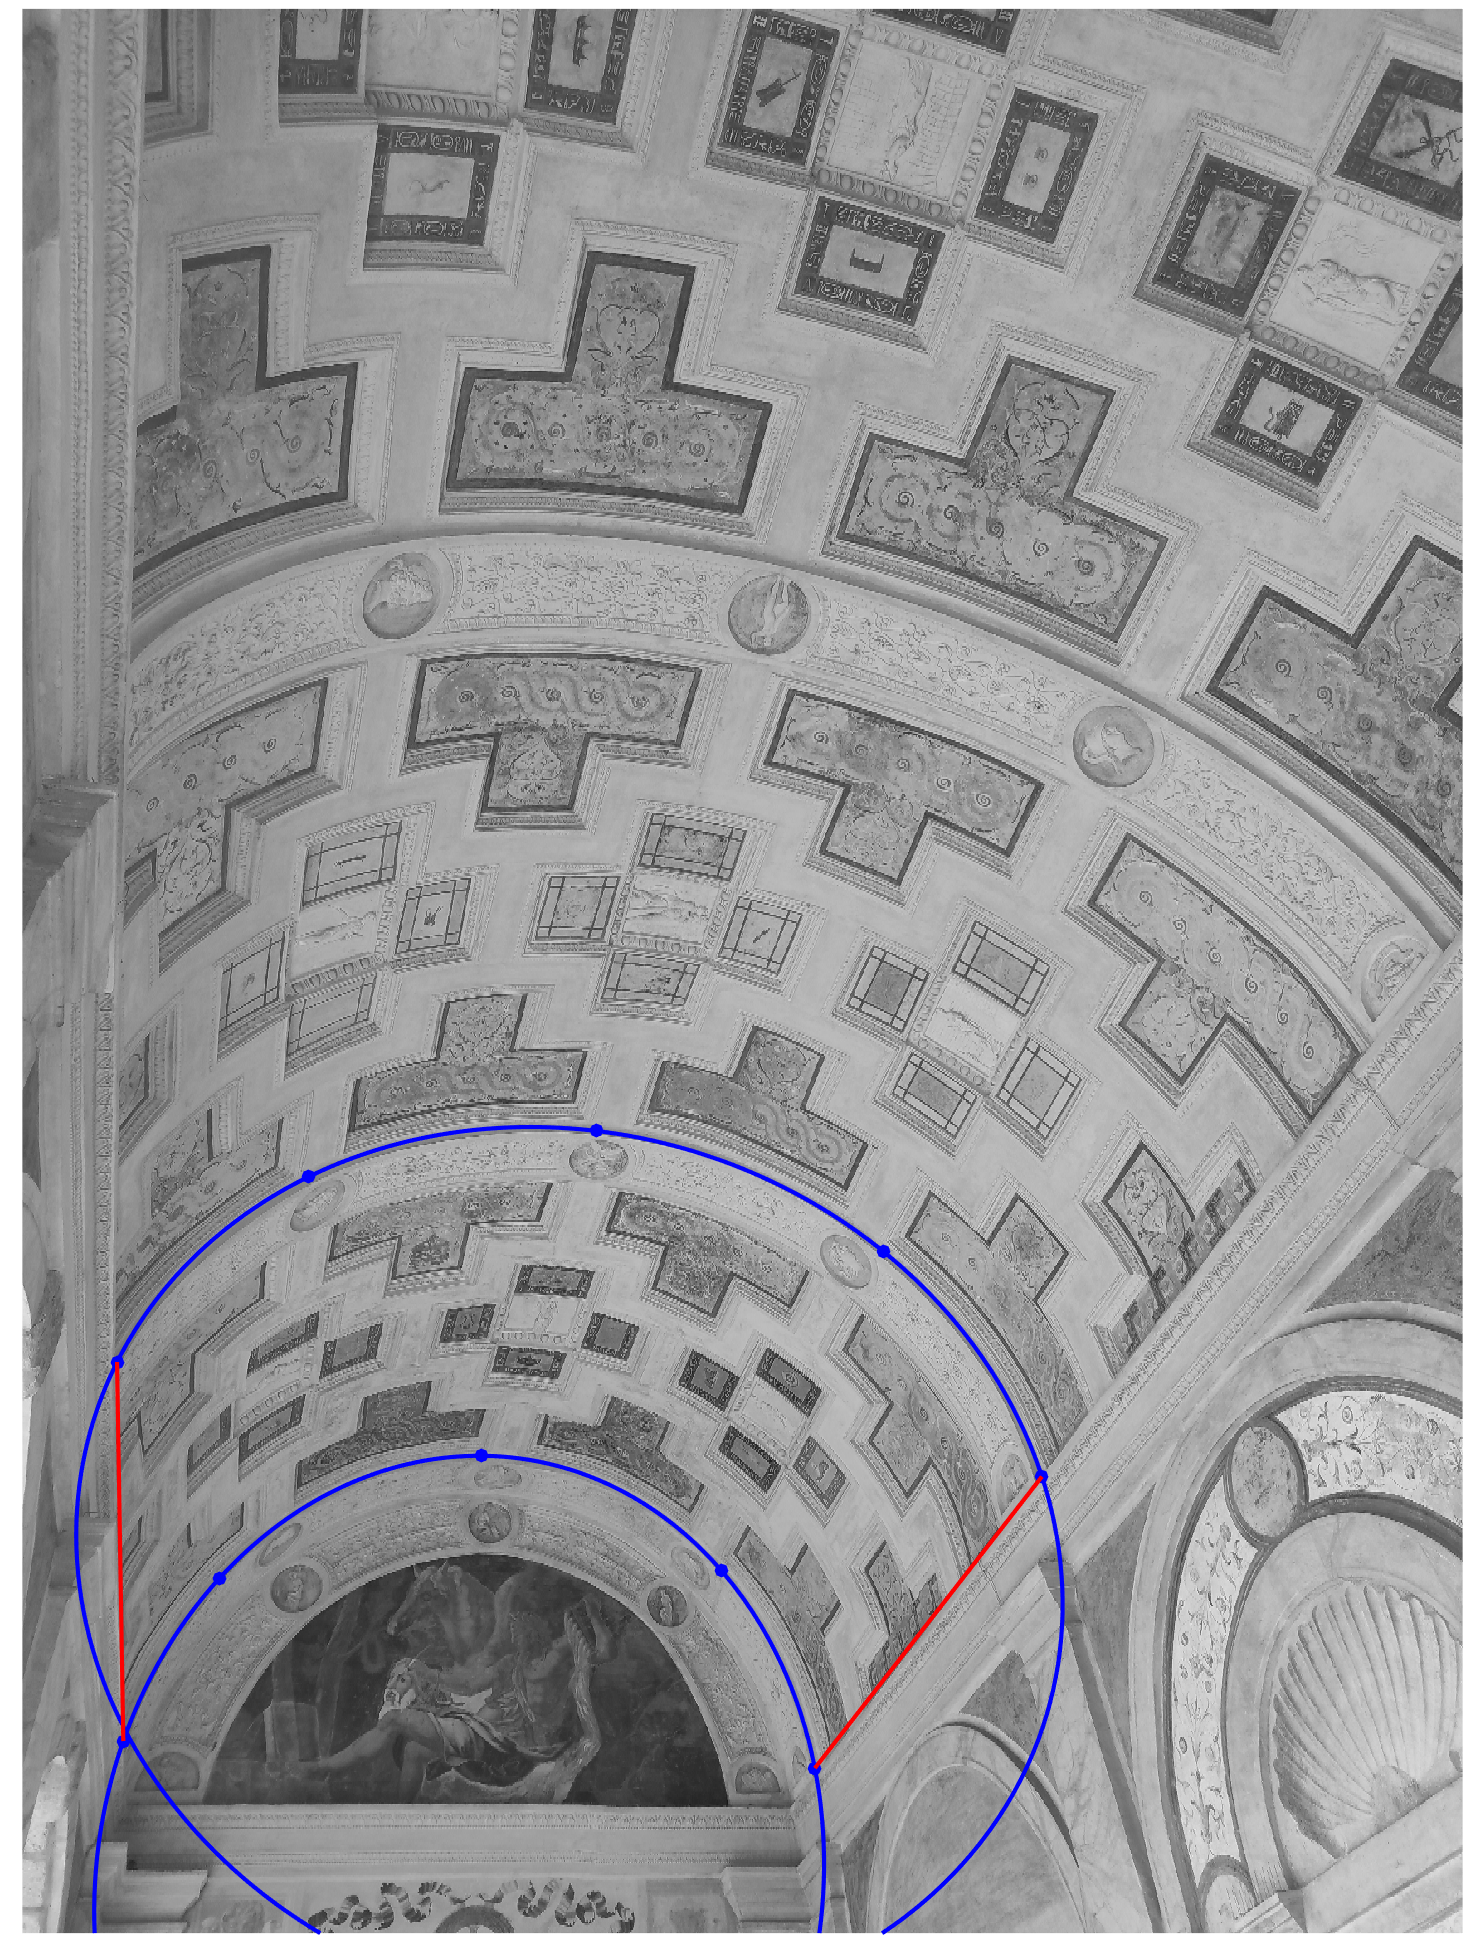
\includegraphics[width=0.73\textwidth]{Images/PalazzoTe_contour.png}
    \caption[Image Contour -- Cross Sections and Generatrix Lines.]{Image Contour -- Cross Sections (blue) and Generatrix Lines (red).}
    \label{fig:contour}
\end{figure}

\subsubsection{Circular Points Image, Vanishing Line}\label{sec:toVanishingLine}
Two conics always intersect in four distinct points in projective geometry. Looking at the two identified cross sections shown in \textbf{Figure \ref{fig:contour}}, it is clear that there are two real intersections and two complex conjugate intersections -- that are exactly the image of circular points.

\begin{minted}{matlab}
% C1,C2 intersections
S = solve(eqns, [x,y]);
s1 = [double(S.x(1));double(S.y(1));1];
s2 = [double(S.x(2));double(S.y(2));1];
s3 = [double(S.x(3));double(S.y(3));1];
s4 = [double(S.x(4));double(S.y(4));1];

% circular points image (complex conjugate pair)
II = s1;
JJ = s2;
\end{minted}

The vanishing line is the line through the image of circular points, and (again) in homogeneous coordinates this amounts to the cross product of the two points. Since the vanishing line equation is computed in homogeneous coordinates, in order to plot the line in the image it is first necessary to convert it in Cartesian coordinates. This can be accomplished by dividing the line vector (in homogeneous coordinates) by the third component. Finally, the line is plotted in the image, as shown in \textbf{Figure \ref{fig:vanishingLine}}.

\begin{minted}{matlab}
% vanishing line
h = cross(II, JJ);
h = h/h(3);
\end{minted}

\begin{figure}[H]
    \centering
    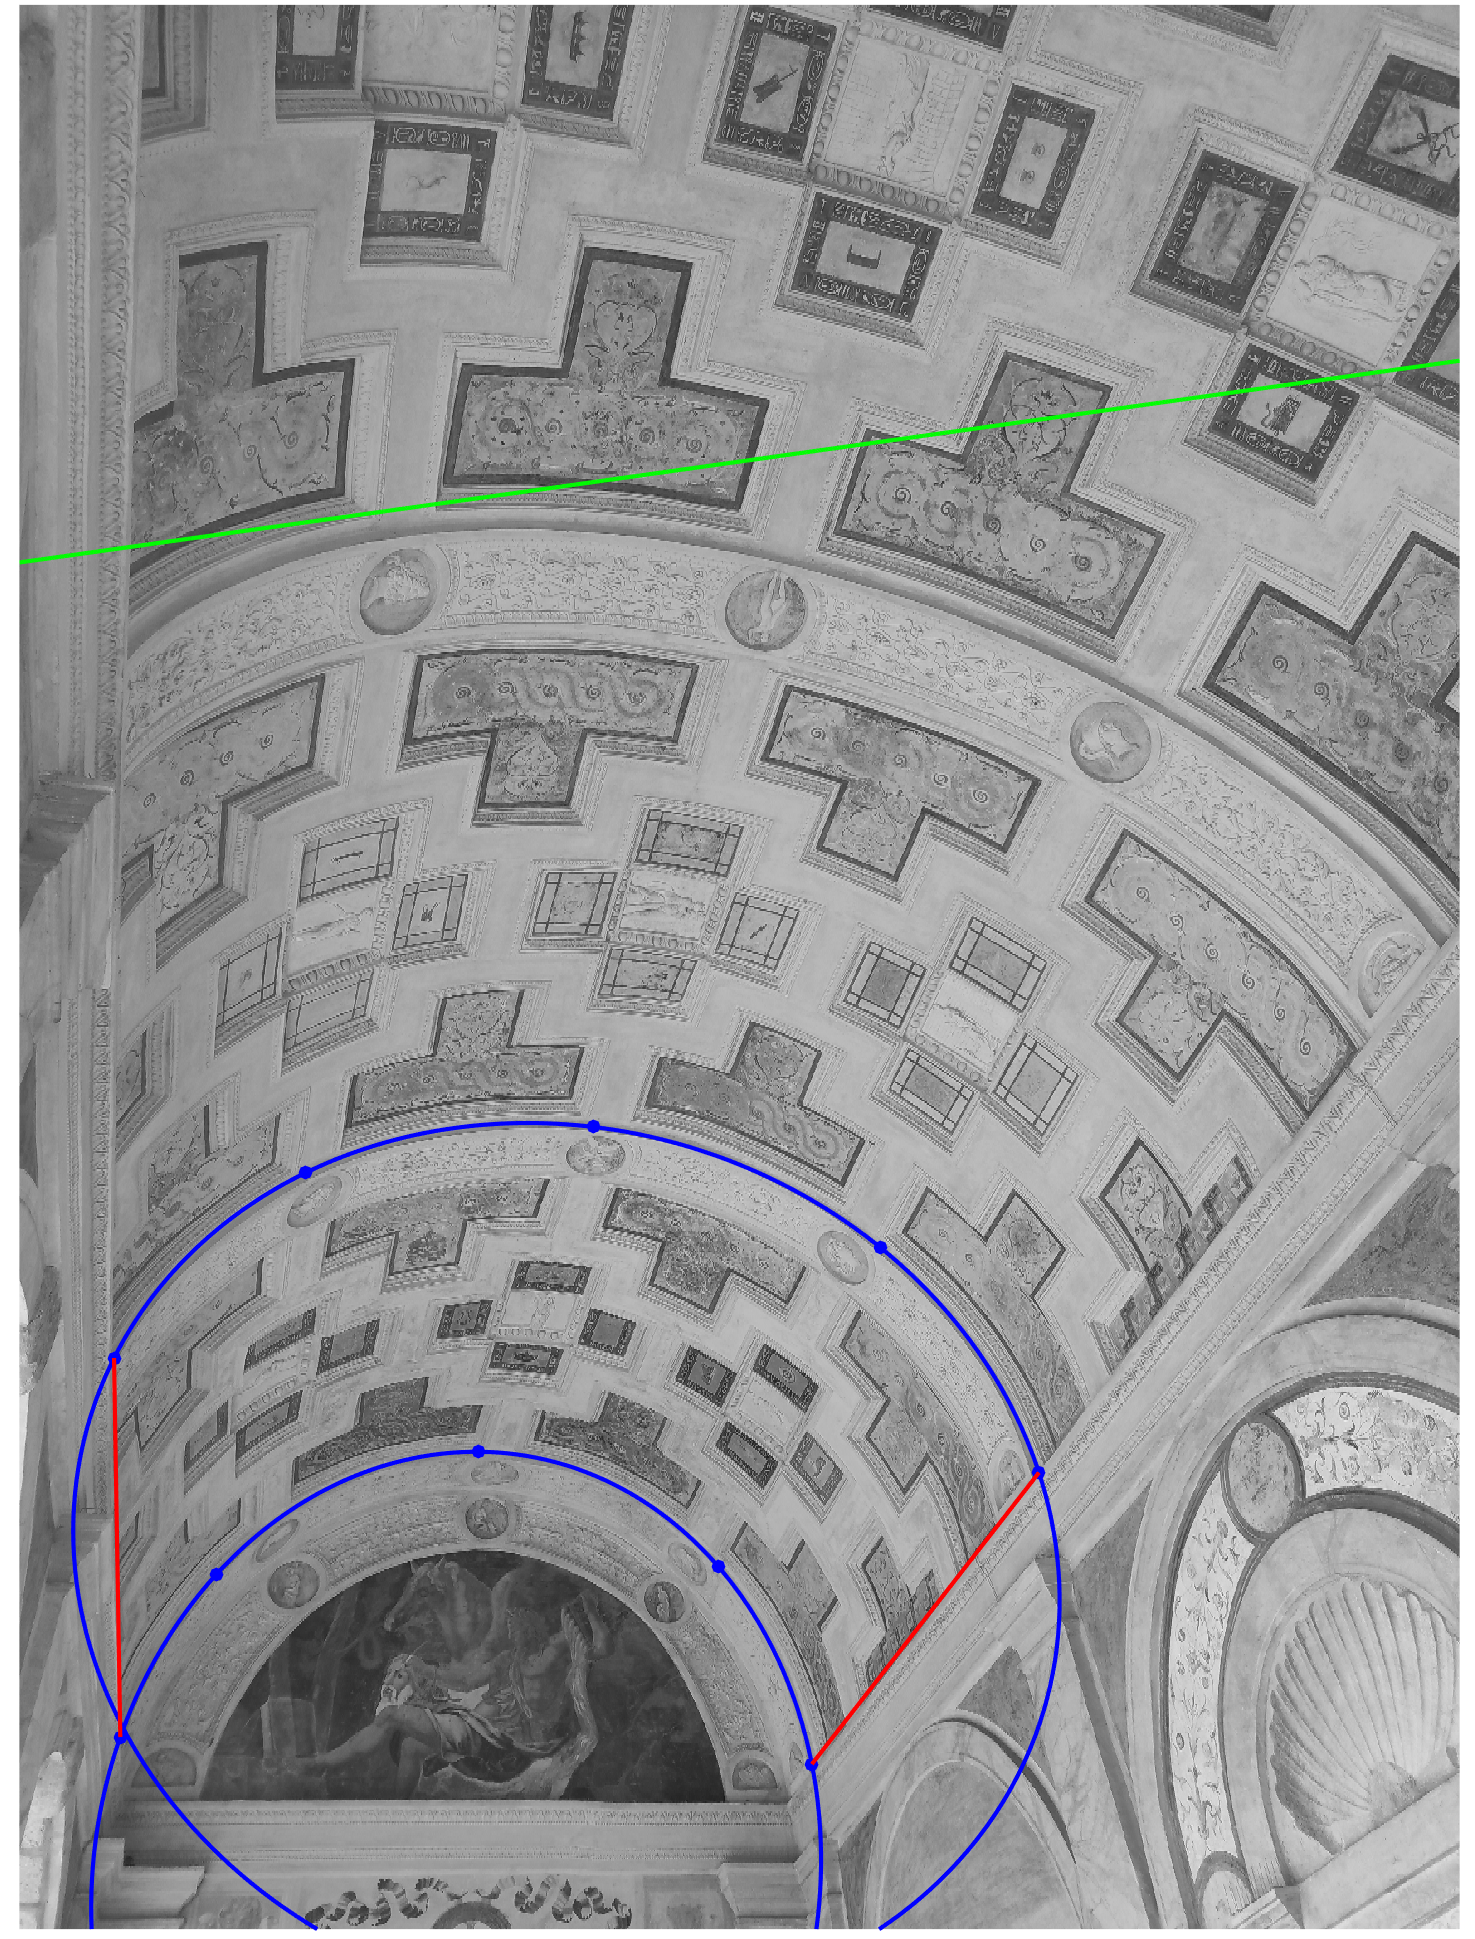
\includegraphics[width=0.73\textwidth]{Images/PalazzoTe_vanishing_line.png}
    \caption[Vanishing Line.]{Vanishing Line (green).}
    \label{fig:vanishingLine}
\end{figure}

\subsubsection{Diameters, Centres, Cylinder Axis Image and Vanishing Point}\label{sec:toAxisImageVanishingPoint}
The diameters are computed multiplying the conics' coefficients matrices with the image of the circular points (two diameters computed per conic).

\begin{minted}{matlab}
% diameters
d1 = C1*II;
d1 = d1/d1(3);
d2 = C1*JJ;
d2 = d2/d2(3);
d3 = C2*II;
d3 = d3/d3(3);
d4 = C2*JJ;
d4 = d4/d4(3);
\end{minted}

For any conic (i.e. image of circular cross section), the intersection point between the two diameters is the center. In homogeneous coordinates this amounts to the cross product of the two lines (i.e. diameters).

\begin{minted}{matlab}
% centres computation
O1 = cross(d1,d2);
O1 = O1./O1(3);
O2 = cross(d3,d4);
O2 = O2./O2(3);

% centres plot
scatter(O1(1), O1(2), 40,'filled','o','MarkerFaceColor','y');
scatter(O2(1), O2(2), 40,'filled','o','MarkerFaceColor','y');
\end{minted}

To retrieve the image of the cylinder axis it suffices to determine the line through the centres of the two cross sections (cross product). The outcome is shown in \textbf{Figure \ref{fig:axisImage}}.

\begin{minted}{matlab}
% cylinder axis image computation
a = cross(O1,O2);

% cylinder axis image plot
x = linspace(1,100000,1000000);
y=((O2(2)-O1(2))/(O2(1)-O1(1)))*(x-O1(1))+O1(2);
plot(x,y,'linewidth',2,'color','c')
\end{minted}

The vanishing point of a given line is the direction (i.e. point at infinity) of the line in the plane. Algebraically, given a line in homogeneous coordinates, it is obtained intersecting it with the canonical line at infinity.

\begin{minted}{matlab}
lInf = [0;0;1];
vp = cross(a,lInf);
vp = vp/vp(3);
\end{minted}

\begin{figure}[H]
    \centering
    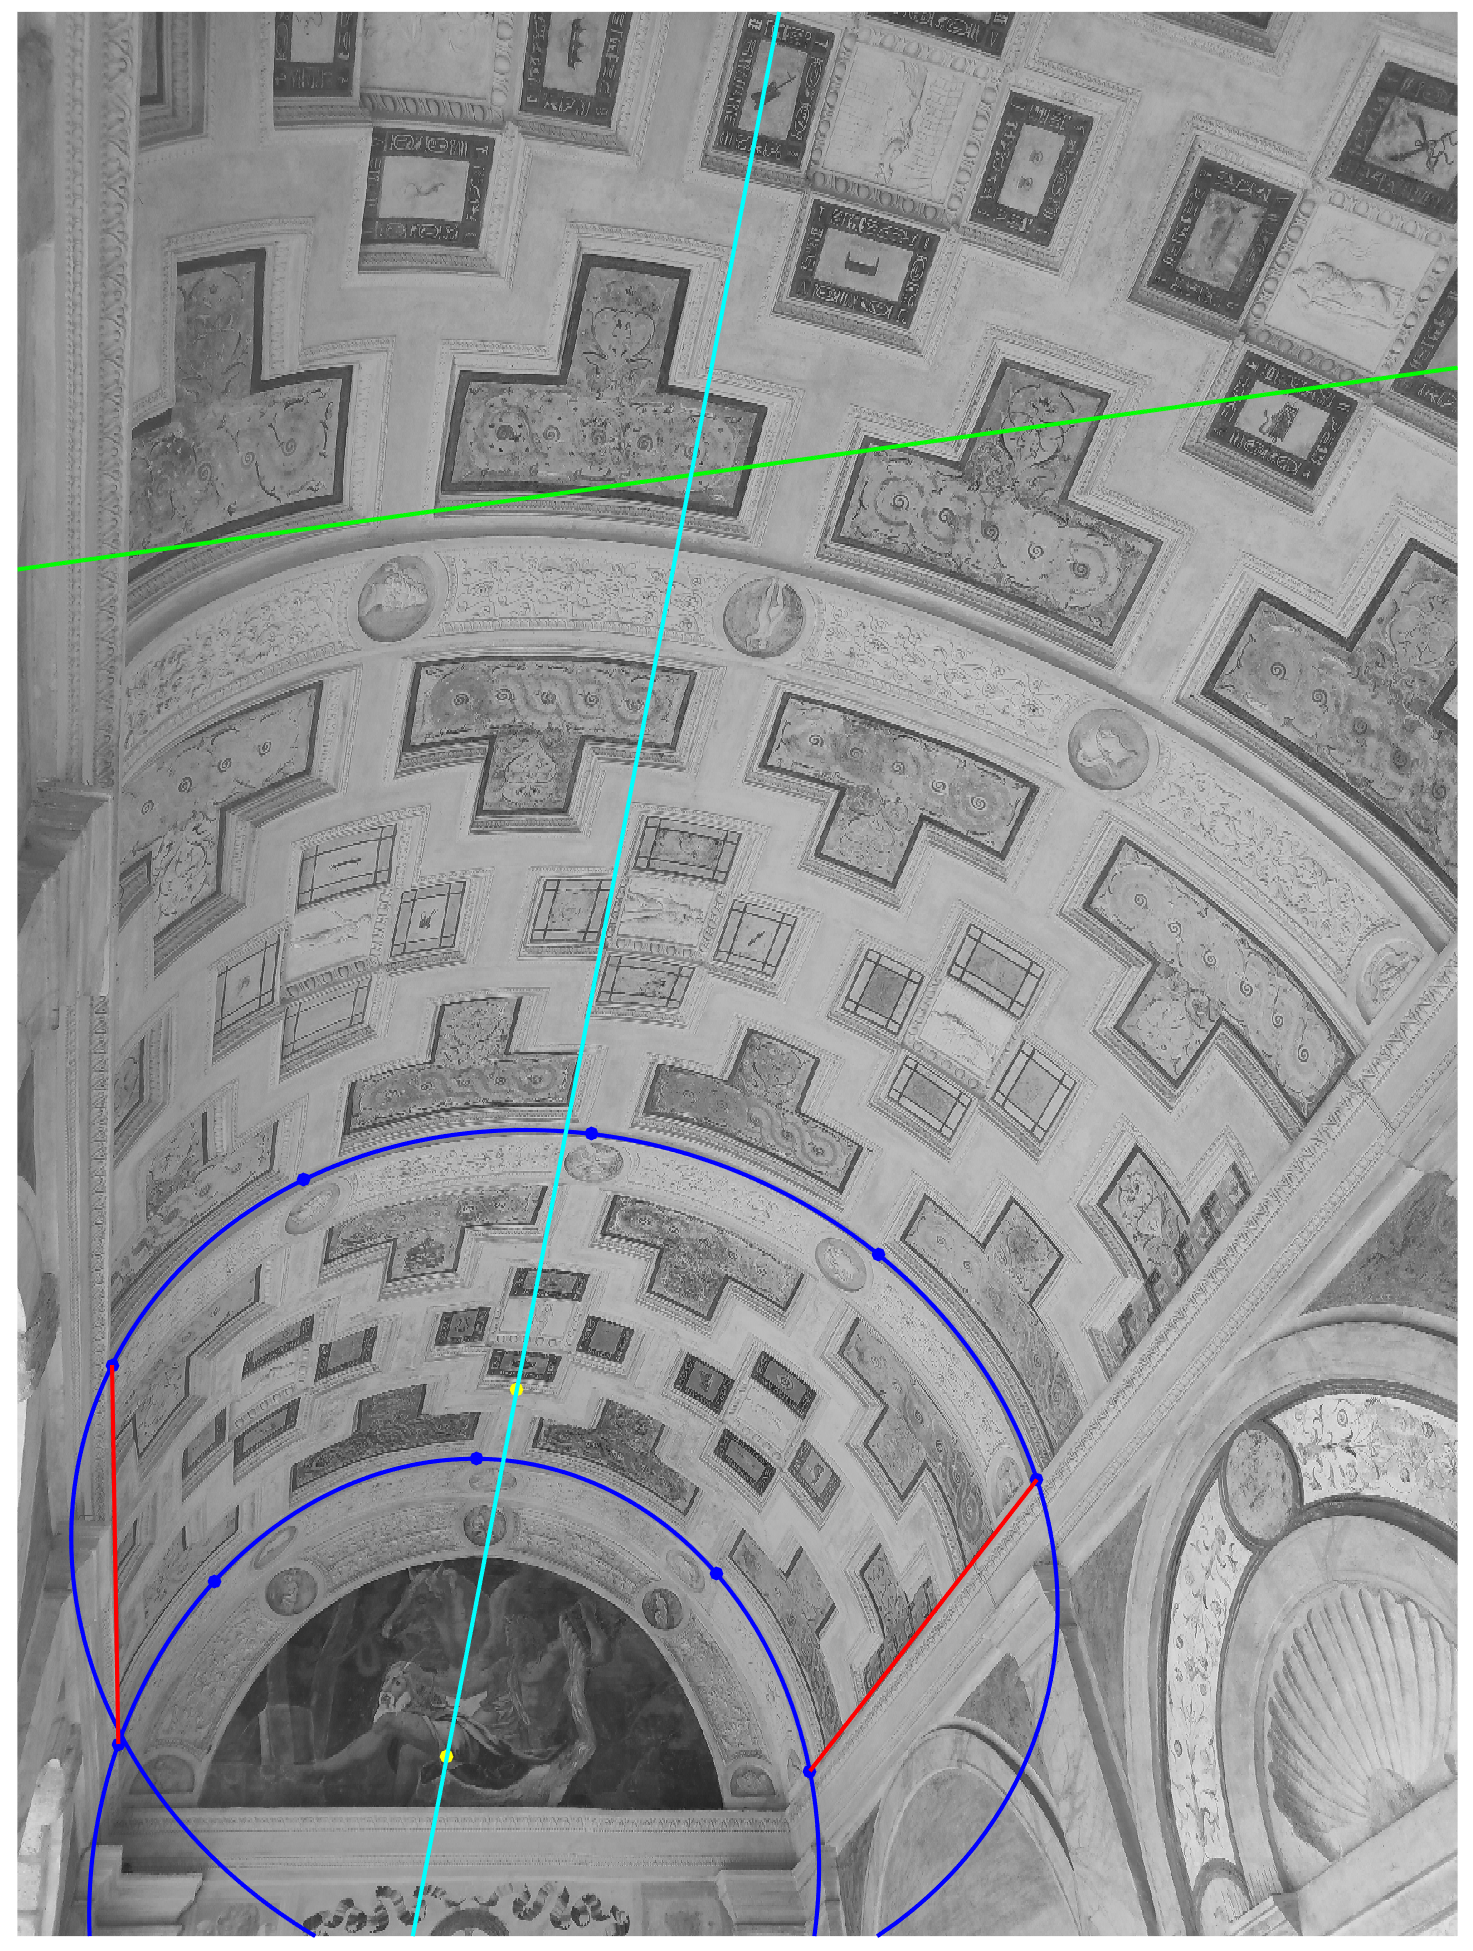
\includegraphics[width=0.73\textwidth]{Images/PalazzoTe_axis.png}
    \caption[Cylinder Axis Image.]{Cylinder Axis Image (cyan).}
    \label{fig:axisImage}
\end{figure}

\subsubsection{Calibration Matrix}\label{sec:toCalibrationMatrix}
In this section, the calibration matrix $K$ -- containing the intrinsic parameters of the camera --  will be computed. In the assignment is stated that the skew factor is null, thus there are four unknowns. Therefore, to estimate the calibration matrix -- using the Image of the Absolute Conic (IAC) -- four constraints (i.e. equations) are necessary. The IAC is strongly related to the camera calibration matrix through the following \textit{Equation \ref{eq:iacCalib}}.

\begin{equation}
    \omega = (KK^T)^{-1} = 
    \begin{bmatrix}
    \alpha^2 & 0 & -U_0\alpha^2\\
    * & 1 & -V_0\\
    * & * & f_Y^2+\alpha^2U_0^2+V_0^2
    \end{bmatrix}
    \label{eq:iacCalib}
\end{equation}
\bigskip

In order to compute the IAC -- using the function \verb|get_IAC| -- three vanishing points were determined, one vertical and two horizontal with respect to the given image.

\pagebreak

The vertical vanishing point has been computed intersecting (using the cross product) two vertical parallel lines (green lines in \textbf{Figure \ref{fig:calibConstraints}}). To find the two horizontal vanishing points, two pairs of parallel lines relying on a horizontal plane were considered (red lines in \textbf{Figure \ref{fig:calibConstraints}}).\\

Using the two horizontal vanishing points, one can compute the image of the line at infinity orthogonal to the vertical vanishing point. This allows to have two constraints with the same equation, because it would be completely equivalent to have two separate constraints using orthogonal vanishing points alone. The other two constraints can be easily recovered exploiting the transformation matrix $H = [h_1,h_2,h_3]$ combined with the image of the circular points $h_1 \pm ih_2$.\\

Hence, the four constraints (three equations) are reported in the system defined by \textit{Equation \ref{eq:calibSystem}}.

\begin{equation}
    \begin{cases}
        l'_\infty = \omega v\\
        h_1^T\omega h_2 = 0\\
        h_1^T\omega h_1 - h_2^T\omega h_2 = 0
    \end{cases}
    \label{eq:calibSystem}
\end{equation}

\begin{figure}[H]
    \centering
    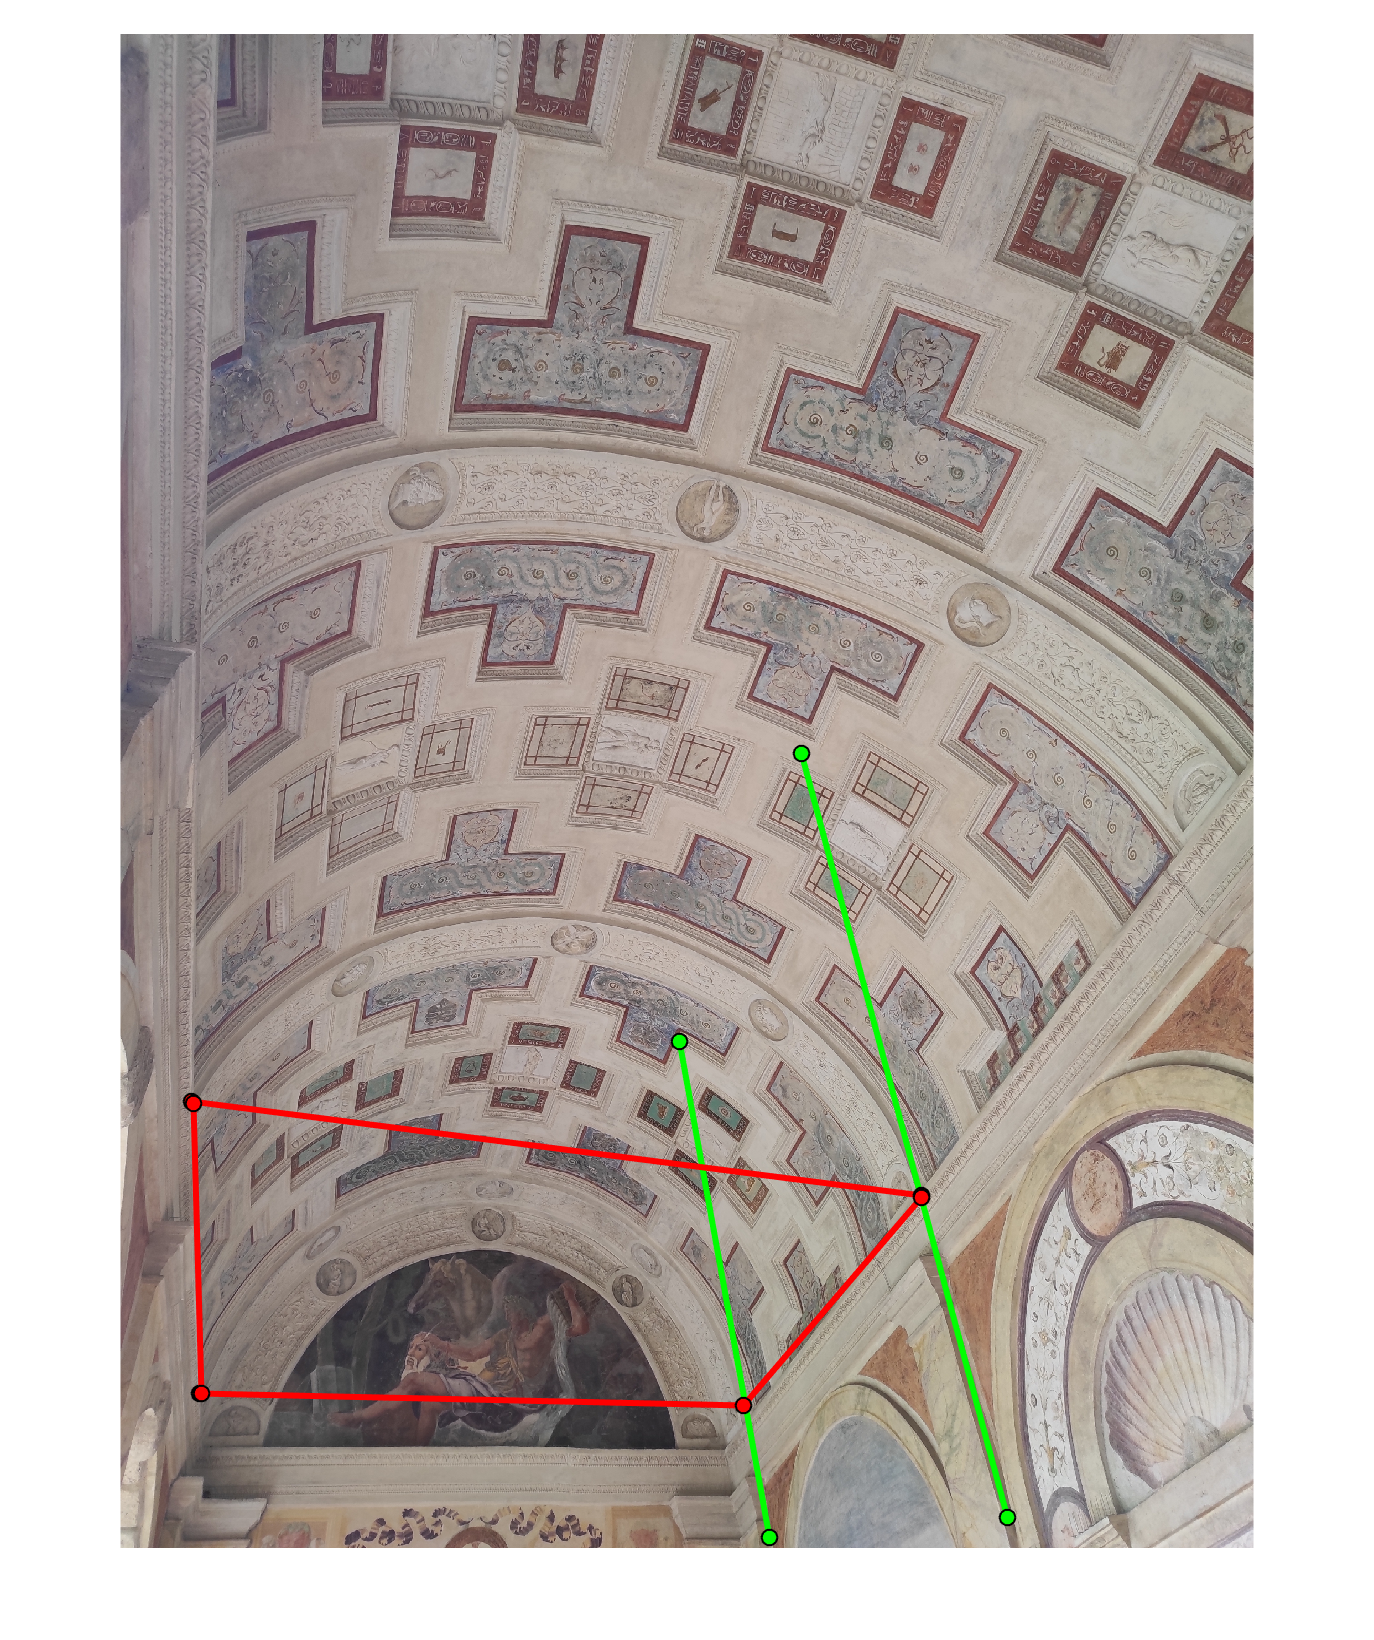
\includegraphics[width=0.83\textwidth]{Images/PalazzoTe_IAC_constraints.png}
    \caption[Calibration Constraints.]{Calibration Constraints.}
    \label{fig:calibConstraints}
\end{figure}

Finally, one can compute the calibration matrix $K$ through Cholesky Decomposition of the IAC. The process is carried out by the following MATLAB code and the obtained calibration matrix is presented in \textit{Equation \ref{eq:calibrationMatrix}}, where $f_X,f_Y,U_0,V_0$ are the camera intrinsic parameters.

\begin{minted}{matlab}
IAC = get_IAC(inf_line, vp1, vp2, vp3, H);
% intrinsic parameters
alfa = sqrt(IAC(1,1));
u0 = -IAC(1,3)/(alfa^2);
v0 = -IAC(2,3);
fy = sqrt(IAC(3,3) - (alfa^2)*(u0^2) - (v0^2));
fx = fy / alfa;
% build K using the parametrization
K = [fx 0 u0; 0 fy v0; 0 0 1];
\end{minted}

\begin{equation}
    K =
    \begin{bmatrix}
    f_X & 0 & U_0\\
    0 & f_Y & V_0\\
    0 & 0 & 1
    \end{bmatrix}
    \approx 10^3
    \begin{bmatrix}
    2.2753 & 0 & 1.0161\\
    0 & 3.8887 & 4.0102\\
    0 & 0 & 1
    \end{bmatrix}
    \label{eq:calibrationMatrix}
\end{equation}
\bigskip

\subsubsection{Cylinder Axis Orientation, Radius-Distance Ratio}\label{sec:toRadiusDistanceRatio}
In this part, the (3D) orientation between the cylinder axis and the camera reference is determined using computed information such as the calibration matrix $K$, the vanishing line $h$, and the vanishing point of the cylinder axis $V$.\\

The process involves transforming the vanishing line $h$ into its corresponding epipolar line $h'$ using the camera calibration matrix $K$, as stated in \textit{Equation \ref{eq:epipolarLine}}.

\begin{equation}
    h' = K^{-T}h
    \label{eq:epipolarLine}
\end{equation}
\bigskip

Subsequently, the direction vector from the camera center to a selected point on the epipolar line is calculated, representing the orientation of the cylinder axis in 3D space. The vanishing point $V$ is projected into 3D space, and the orientation of the cylinder axis is determined by the cross product of the direction vector and the 3D coordinates of the projected vanishing point. The resulting direction vector is then normalized to represent the unit vector along the axis.\\

Optional visualizations, such as plotting the vanishing line and the direction vector on the image, provide additional insights into the cylinder axis orientation.\\

The following MATLAB code summarizes the explained process.

\begin{minted}{matlab}
% transform vanishing line l to epipolar line l'
h_prime = inv(K)' * h;

% find the intersection point P of l' with the image plane
P = cross(h_prime, [1; 0; 0]);  % assuming x-axis as principal axis

% calculate the direction vector from the camera center to P
C = -inv(K) * h;  % camera center
direction_vector = (P - C) / norm(P - C); % orientation of the cylinder axis

% display result (3D)
% orientation rotation matrix
R = direction_vector;
[U, ~, V] = svd(R);
R = U * V';
axis_orientation = R.';
poseplot(axis_orientation);
\end{minted}

\begin{figure}[H]
    \centering
    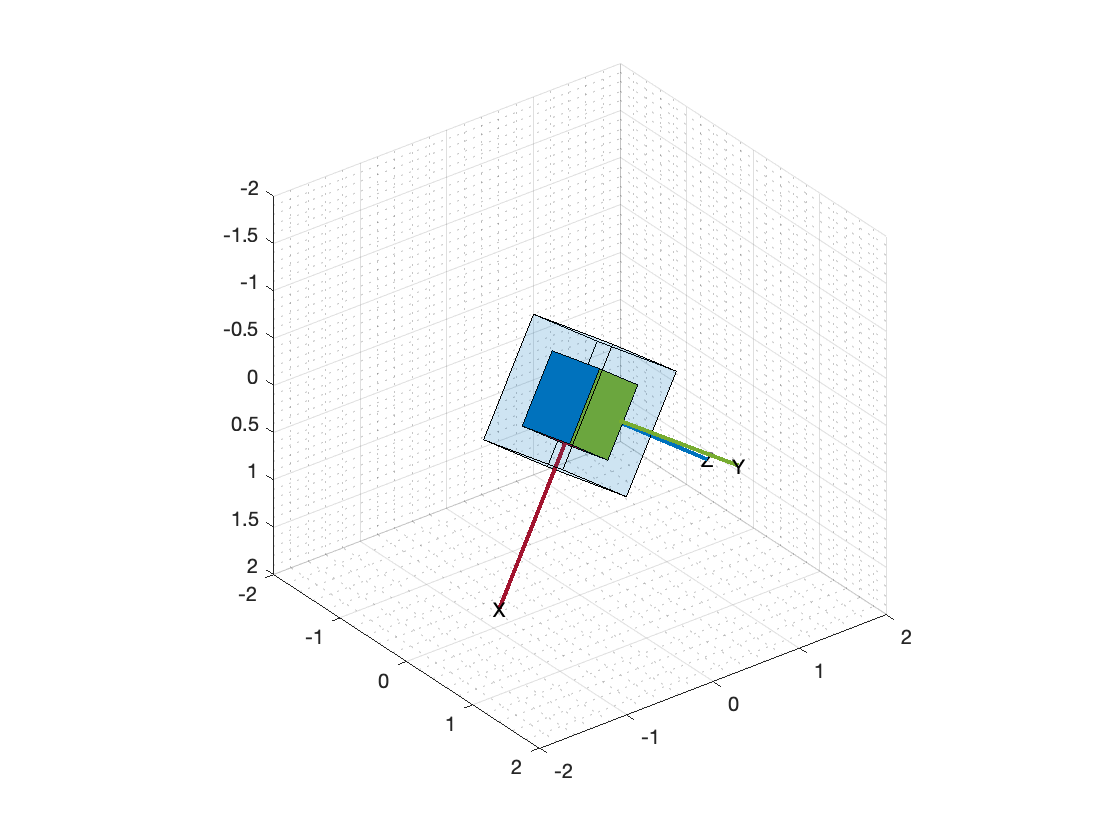
\includegraphics[width=0.83\textwidth]{Images/axis_orientation.png}
    \cprotect\caption[Cylinder Axis Orientation.]{Cylinder Axis Orientation (red) and Vanishing Line (green) -- plotted in 3D using \verb|poseplot|.}
    \label{fig:axisImage}
\end{figure}

Finally, the radius-distance ratio is computed using known parameters such as generic points on the conics and their centres. Specifically, the Euclidean distance between desired endpoints is determined using MATLAB \verb|pdist| function. The ratio -- considering the less distorted conic --  is approximately unitary.

\begin{minted}{matlab}
% compute cross section radius
radiusC1 = pdist([p1(1),p1(2);O1(1),O1(2)], 'euclidean'); % less distorted
radiusC2 = pdist([p3(1),p3(2);O2(1),O2(2)], 'euclidean');

% compute distance between cross sections (centers)
distance = pdist([O1(1),O1(2);O2(1),O2(2)], 'euclidean');

% compute ratio
ratio1 = radiusC1/distance; % 1.0991 (computed result)
ratio2 = radiusC2/distance; % 1.5525 (computed result)
\end{minted}

\pagebreak

\subsection{Metric Rectification}
\label{sec:shapeReconstruction}
The objective is to metric rectify (i.e. 2D reconstruct) the unfolding of the part of the cylinder surface included between the two cross sections onto a plane.\\

Metric rectification will be accomplished using images of circles \cite{MetRecCircles}. Specifically, three images of circles will be used, as shown in \textbf{Figure \ref{fig:recConics}}. To determine the parameters of the selected conics, the same method used to estimate the cross sections has been used.

\begin{figure}[H]
    \centering
    \includegraphics[width=1\textwidth]{Images/PalazzoTe_rec_conics.png}
    \caption[Circles Images used for Rectification.]{Circles Images used for Rectification.}
    \label{fig:recConics}
\end{figure}

Then, for every pair of conics the intersections are computed. In order to disambiguate between the solutions the image of the circular points is determined as the mean one among the ones computed. Next, the line at infinity is computed using the image of the conic dual to the circular points -- that is determined using the definition. The affine rectification matrix is evaluated using the line at infinity, as shown in \textit{Equation \ref{eq:hMatrix}}.

\begin{equation}
    H = 
    \begin{bmatrix}
    1 & 0 & 0\\
    0 & 1 & 0\\
    & {l'_\infty}^T &
    \end{bmatrix}
    \label{eq:hMatrix}
\end{equation}
\bigskip

At this point, taken one of the three conics (e.g. $C_1$) its projective transformation in the rectified plane is obtained applying the rule stated in \textit{Equation \ref{eq:qMatrix}}.

\begin{equation}
    Q = H^{-T}C_1H^{-1}
    \label{eq:qMatrix}
\end{equation}
\bigskip

Using implemented MATLAB function \verb|AtoG| one can extract geometric information about the conic on the rectified plane (i.e. $Q$) from its (known) parameters.\\

To compute the affinity that rectifies the cylinder, the idea is to build the one that makes the axis of the ellipses to be equal (i.e. maps the conic in the image onto a circle in the rectified image). To do this, the desired affinity is obtained combining a rotation -- using rotation matrix $U$ defined in \textit{Equation \ref{eq:uMatrix}} -- and a scaling -- using diagonal matrix $S$ defined in \textit{Equation \ref{eq:sMatrix}}, which rescales the axis to be unitary.\\

\begin{equation}
    U = 
    \begin{bmatrix}
    cos(\alpha) & -sin(\alpha)\\
    sin(\alpha) & cos(\alpha)
    \end{bmatrix}
    \label{eq:uMatrix}
\end{equation}
\bigskip
\begin{equation}
    S = 
    \begin{bmatrix}
    1 & 0\\
    0 & a/b
    \end{bmatrix}
    \label{eq:sMatrix}
\end{equation}
\bigskip

The final transformation $T$ is the composition between the homography that maps the image of the line at infinity to its canonical position and the rescaling homography, and is computed as stated in the following \textit{Equations \ref{eq:kMatrix}, \ref{eq:aMatrix}, \ref{eq:tMatrix}}. Eventually, the rectified cylinder surface unfolded onto a plane is shown in \textbf{Figure \ref{fig:rectified}}.

\begin{equation}
    K = USU^T
    \label{eq:kMatrix}
\end{equation}

\begin{equation}
    A = 
    \begin{bmatrix}
    K & 0_{2x1}\\
    0_{1x2} & 1
    \end{bmatrix}
    \label{eq:aMatrix}
\end{equation}

\begin{equation}
    T = AH
    \label{eq:tMatrix}
\end{equation}
\bigskip

The following MATLAB code carries out the outlined procedure.

\begin{minted}{matlab}
imDCCP = II*JJ' + JJ*II';
imDCCP = imDCCP./norm(imDCCP);
l_inf = null(imDCCP);
H = [eye(2), zeros(2,1); l_inf(:)'];

% conic projective transformation
Q = inv(H)'*C1*inv(H);
Q = Q./Q(3,3);

% conic geometric information extraction
par_geo = AtoG([Q(1,1),2*Q(1,2),Q(2,2),2*Q(1,3),2*Q(2,3),Q(3,3)]);
center = par_geo(1:2);
axes = par_geo(3:4);
a = axes(1);
b = axes(2);
alpha = par_geo(5);

% rotation and scaling
U = [cos(alpha), -sin(alpha); sin(alpha), cos(alpha)];
S = diag([1, a/b]);

% composition homography
K = U*S*U';
A = [K zeros(2,1); zeros(1,2), 1];
T = A*H;
tform = projective2d(T');
J = imwarp(img, tform);
\end{minted}

\begin{figure}[H]
    \centering
    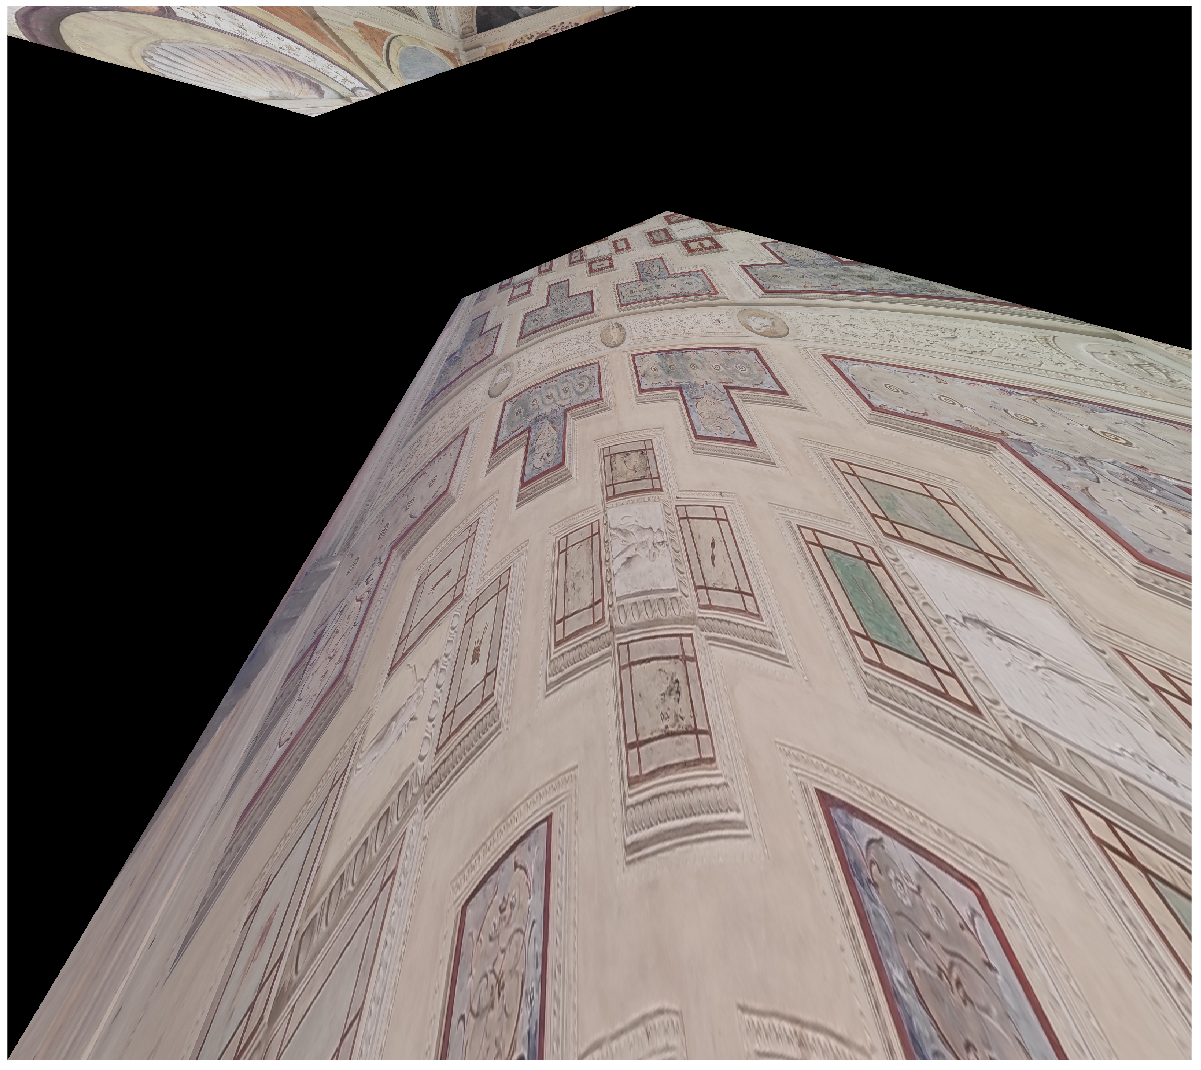
\includegraphics[width=1\textwidth]{Images/PalazzoTe_rectified.png}
    \caption[Rectified Cylinder Surface between two Cross Sections.]{Rectified Cylinder Surface between two Cross Sections.}
    \label{fig:rectified}
\end{figure}

\pagebreak

\section*{Directory Tree}

\begin{forest}
      for tree={
        font=\ttfamily,
        grow'=0,
        child anchor=west,
        parent anchor=south,
        anchor=west,
        calign=first,
        inner xsep=7pt,
        edge path={
          \noexpand\path [draw, \forestoption{edge}]
          (!u.south west) +(7.5pt,0) |- (.child anchor) pic {folder} \forestoption{edge label};
        },
        % style for your file node 
        file/.style={edge path={\noexpand\path [draw, \forestoption{edge}]
          (!u.south west) +(7.5pt,0) |- (.child anchor) \forestoption{edge label};},
          inner xsep=2pt,font=\small\ttfamily
                     },
        before typesetting nodes={
          if n=1
            {insert before={[,phantom]}}
            {}
        },
        fit=band,
        before computing xy={l=15pt},
      }  
    [Versiglioni-Giovanni
      [docs
        [Report.pdf,file
        ]
      ]
      [img
        [1 - Feature Extraction
        ]
        [2 - Rectification
        ]
      ]
      [src
        [1 - Feature Extraction
            [detectCorners.m,file
            ]
            [detectEdges.m,file
            ]
            [detectLines.m,file
            ]
            [Functions
            ]
        ]
        [2 - Rectification
            [Problems.m,file
            ]
            [Rectification.m,file
            ]
            [Functions
            ]
        ]
      ]
    ]
 \end{forest}

 \vspace{1.5cm}

 The homework report is accessible via the \verb|Report.pdf| file.\\

 The used input image and the output images (with respect to both feature extraction and rectification) are inside the \verb|img| folder.\\

 The MATLAB code responsible of extracting features from the image is distributed among the \verb|detectCorners.m|, \verb|detectEdges.m|, and \verb|detectLines.m| scripts. Functions used/implemented are also included.\\

 The MATLAB code containing the detailed solutions to Problems 1-5 is in the \verb|Problems.m| script, while the rectification of the cylinder surface is in the \verb|Rectification.m| script. Functions used/implemented are also included.

\pagebreak

\section*{Matlab Functions}

\begin{minted}{matlab}
function [corner_x, corner_y] = findCorners(I, sigma, border_margin)
    dx = [-1 0 1; 
          -1 0 1; 
          -1 0 1];
    dy = dx';
    Ix = conv2(I, dx, 'same');
    Iy = conv2(I, dy, 'same');
    g = fspecial('gaussian', max(1,fix(3*sigma)+1), sigma);
    Ix2 = conv2(Ix.^2, g, 'same');
    Iy2 = conv2(Iy.^2, g, 'same');
    Ixy = conv2(Ix.*Iy, g, 'same');
    cm = (Ix2.*Iy2 - Ixy.^2)./(Ix2 + Iy2 + eps);
    cm(1:border_margin,:) = 0;
    cm(end-border_margin:end,:) = 0;
    cm(:,end-border_margin:end) = 0;
    cm(:,1:border_margin) = 0;
    T = mean(cm(:));
    CIM = cm;
    CIM(cm<T) = 0;
    support = true(11);
    maxima = ordfilt2(CIM, sum(support(:)), support);
    [corner_x, corner_y] = find((cm==maxima).*(CIM>0));
end
\end{minted}

\begin{minted}{matlab}
function lines = findLines(I)
    edges = edge(I, 'canny', [0.2 0.25]);
    [H,T,R] = hough(edges);
    P = houghpeaks(H, 100, 'threshold', 0.3*max(H(:)));
    lines = houghlines(edges, T, R, P, 'FillGap', 200, 'MinLength', 500);
end
\end{minted}

\begin{minted}{matlab}
function [l] = segToLine(pts)
    a = [pts(1,:)';1];
    b = [pts(2,:)';1];
    l = cross(a,b);
    l = l./norm(l);
end
\end{minted}

\begin{minted}{matlab}
function IAC = get_IAC(l_infs, vps, vp1s, vp2s, H)
% Returns the Image of the absolute conic
% Full code in '2 - Rectification/Functions'
end
\end{minted}

\begin{minted}{matlab}
function [ParG,code] = AtoG(ParA)
% Conversion of algebraic parameters to geometric parameters
% ParG = [Center(1:2), Axes(1:2), Angle]'
% Full code in '2 - Rectification/Functions'
end
\end{minted}

\pagebreak

\bibliography{bibliography.bib}

\end{document}
% DOUMENT END
